\PassOptionsToPackage{table}{xcolor}
\documentclass{article}
\usepackage{iclr2026_conference,times}

% to avoid loading the natbib package, add option nonatbib:
%    \usepackage[nonatbib]{iclr2026_conference}

\usepackage[utf8]{inputenc}
\usepackage[T1]{fontenc}
\usepackage[pagebackref,breaklinks,colorlinks]{hyperref}
\usepackage{url}
\usepackage{booktabs}
\usepackage{makecell}
\usepackage{enumitem}
\usepackage{amsmath,amssymb,amsfonts,mathtools}
\usepackage{amsthm}
\usepackage{nicefrac}
\usepackage{microtype}
\usepackage{colortbl}
\usepackage{latexsym}
\usepackage{float}
\usepackage{graphicx}
\usepackage{multirow}
\usepackage{inconsolata}
\usepackage{tikz}
\usetikzlibrary{positioning,calc,arrows.meta,shadows}
\usepackage{caption}
\usepackage{subcaption}
\usepackage{tabularx}
\usepackage[most]{tcolorbox}
\tcbuselibrary{raster,skins,listings,breakable}
\usepackage{adjustbox}
\usepackage{placeins}
\usepackage{pifont}
\usepackage{array}
\usepackage{fontawesome5}
\usepackage{fancyhdr}
\usepackage{wrapfig}
\usepackage[capitalize,noabbrev]{cleveref}
\usepackage{etoc}
\usepackage{titletoc}
\usepackage[leftmargin=1em, rightmargin=1em, indentfirst=false]{quoting}

% -----------------------------------------------------------------------
% Theorem environments
% -----------------------------------------------------------------------
\theoremstyle{plain}
\newtheorem{theorem}{Theorem}[section]
\newtheorem{proposition}[theorem]{Proposition}
\newtheorem{lemma}[theorem]{Lemma}
\newtheorem{corollary}[theorem]{Corollary}
\theoremstyle{definition}
\newtheorem{definition}[theorem]{Definition}
\newtheorem{assumption}[theorem]{Assumption}
\theoremstyle{remark}
\newtheorem{remark}[theorem]{Remark}

% -----------------------------------------------------------------------
% Math commands
% -----------------------------------------------------------------------
\input{math_commands.tex}

% -----------------------------------------------------------------------
% Color definitions
% -----------------------------------------------------------------------
\definecolor{valbest}{HTML}{d9ead3}
\newcommand{\valbest}[1]{\colorbox{valbest}{#1}}
\definecolor{valgood}{HTML}{cfe6ec}
\newcommand{\valgood}[1]{\colorbox{valgood}{#1}}
\definecolor{valmid}{HTML}{fce5cd}
\newcommand{\valmid}[1]{\colorbox{valmid}{#1}}
\definecolor{valbad}{HTML}{ead1dc}
\newcommand{\valbad}[1]{\colorbox{valbad}{#1}}
\definecolor{llamiabench}{HTML}{D8D4F2}
\newcommand{\llamiabench}[1]{\colorbox{llamiabench}{#1}}

\definecolor{themegreen}{HTML}{365956}
\definecolor{themepurple}{HTML}{3c1b48}
\definecolor{themered}{HTML}{b43748}

% -----------------------------------------------------------------------
% State / Language / Action macros
% -----------------------------------------------------------------------
\definecolor{StateColor}{HTML}{F94892}
\definecolor{LanguageColor}{HTML}{FF7F3F}
\definecolor{ActionColor}{HTML}{02B9F1}

\newcommand{\state}[1]{\textcolor{StateColor}{\textbf{#1}}}
\newcommand{\lang}[1]{\textcolor{LanguageColor}{\textbf{#1}}}
\newcommand{\action}[1]{\textcolor{ActionColor}{\textbf{#1}}}
\newcommand{\mstate}[1]{{\color{StateColor}#1}}
\newcommand{\mlang}[1]{{\color{LanguageColor}#1}}
\newcommand{\maction}[1]{{\color{ActionColor}#1}}
\newcommand*\circled[1]{\tikz[baseline=(char.base)]{
            \node[shape=circle,draw,inner sep=0.8pt] (char) {#1};}}

% -----------------------------------------------------------------------
% Collaborative annotation macros (suppress in submission)
% -----------------------------------------------------------------------
\newcommand{\somesh}[1]{}
\newcommand{\yaman}[1]{}
\newcommand{\harini}[1]{}

% -----------------------------------------------------------------------
% Suppress ACM \Description{} — not defined in ICLR template
% -----------------------------------------------------------------------
\providecommand{\Description}[1]{}

% -----------------------------------------------------------------------
% Institution logo macros
% -----------------------------------------------------------------------
\DeclareRobustCommand{\coauth}{$^*$}
\DeclareRobustCommand{\adobelogo}{%
  \raisebox{0.15\height}{
\includegraphics[height=2ex]{images/adobe-logo.png}}}
\DeclareRobustCommand{\iiitdlogo}{%
  \raisebox{0.25\height}{
\includegraphics[height=1.2ex]{images/iiitd-logo.png}}}
\DeclareRobustCommand{\ublogo}{%
  \raisebox{0.25\height}{
\includegraphics[height=1.2ex]{images/ub-logo.png}}}
\newcommand{\auth}[2]{\textbf{#1}~#2}

\newcommand\blfootnote[1]{%
  \begingroup
  \renewcommand\thefootnote{}\footnote{#1}%
  \addtocounter{footnote}{-1}%
  \endgroup
}
\newcommand{\cmark}{\textcolor{green!60!black}{$\checkmark$}}
\newcommand{\xmark}{\textcolor{red!70!black}{\texttimes}}

% -----------------------------------------------------------------------
\title{Exploring Collaboration between a language and a non-language agent}

\author{%
\parbox{\textwidth}{\centering\vspace{4mm}
\renewcommand{\arraystretch}{1.35}
\setlength{\tabcolsep}{6pt}
\begin{tabular}{@{}ccc@{}}
  \auth{Harini S I\coauth}{\adobelogo} &
  \auth{Somesh Singh\coauth}{\adobelogo~\iiitdlogo~\ublogo} &
  \auth{Yaman K Singla}{\adobelogo} \\
\end{tabular}\\[1.5mm]
\begin{tabular}{@{}ccc@{}}
  \auth{Rajiv Ratn Shah}{\iiitdlogo} &
  \auth{David Doermann}{\ublogo} &
  \auth{Balaji Krishnamurthy}{\adobelogo} \\[3mm]
\end{tabular}\\
{\adobelogo~Adobe Media and Data Science Research (MDSR)\\[0.5mm]
 \iiitdlogo~IIIT-Delhi,\quad \ublogo~SUNY at Buffalo\\[1mm]}
\small\faEnvelope\ \texttt{\href{mailto:behavior-in-the-wild@googlegroups.com}{behavior-in-the-wild@googlegroups.com}}
}%
}

% -----------------------------------------------------------------------
% Page header
% -----------------------------------------------------------------------
\pagestyle{fancy}
\fancyhf{}
\setlength{\headheight}{13pt}
\fancyhead[L]{%
  \raisebox{0.01\height}{%
    
\includegraphics[height=2ex]{images/adobe-logo.png}%
  }\hspace{0.1em}%
  Adobe Media and Data Science Research
}
\renewcommand{\headrulewidth}{0.4pt}
\renewcommand{\footrulewidth}{0pt}

\iclrfinalcopy  % remove this line for anonymous submission

\begin{document}

\maketitle

\begin{abstract}
  LLMs are increasingly deployed as orchestrators that coordinate specialized subagents
  to solve complex tasks through natural language. However, in many important domains like game playing and robotics
  the strongest available agents are not language models. Integrating non language agents with LLMs would require \emph{verbalization} or compressing their rich continuous representations into sparse textual summaries at each interaction step.
  In this work we introduce the concept of \textit{latent state internalization}: instead of verbalizing the non language agent's state, we project its internal continuous representations directly into the LLM's chain of thought as learned state tokens. We show that training LLMs and subagents through internalization and reinforcement learning can solve previously unsolvable tasks, and a single model can outperform existing state of the art task specific methods trained over 100$\times$ more data.
  To evaluate these collaborative abilities, we introduce \textsc{LLAMIA-Bench}, a suite of six collaborative chess tasks from prominent AI literature spanning: behavior cloning, state understanding, and natural-language explanation of actions and policies. These tasks cannot be solved by LLMs or subagents independently, making them a perfect testbed for studying collaboration. Our experiments reveal a consistent \emph{verbalization debt}:
  verbalizing the subagent's state consistently trails internalizing it, and this gap does not shrink as the LLM scales from 4B to 14B parameters. A single 14B model,
  \textsc{LLAMIA}, trained under this paradigm matches or exceeds both dedicated task specific trained models and the strongest verbalization-based pipeline, GPT-5.1 with tool access, across all benchmark tasks.
\end{abstract}

\begin{NoHyper}
    \blfootnote{\coauth \small Equal Contribution.}
\end{NoHyper}


\section{Introduction}
Large language models (LLMs) are increasingly deployed as general-purpose orchestrators that coordinate tools and agents to solve complex tasks \citep{hong_metagpt_2024, tran_multi-agent_2025}.
A central pattern in this paradigm is collaboration with \emph{subagents} or agents that excel within a narrow domain ~\cite{anthropic_claude_subagents_2025,openai_codex_subagents_2025}.
This collaboration allows orchestrator LLMs to utilize the subagent's domain specific intelligence \citep{hong_metagpt_2024} and preserve its context length by task delegation \citep{zhang_chain_2024}, enabling effective multi-step reasoning and planning over long horizons.
Today, this collaboration is mediated entirely through natural language: the LLM invokes the subagent, receives a natural language description of its output, and reasons over that description to decide subsequent actions\citep{tran_multi-agent_2025}. 
Natural language collaboration is reasonable when both agents are themselves language models, as they share the same input space. 
However, in many important domains such as game playing, robotics, and  autonomous driving the strongest available agents are not language models; their expertise is encoded in internal representations: latent states capturing policy, value estimates, and learned features~\cite{silver2017mastering,monroe2024mastering,brohan2022rt}.
This mismatch between LLMs and non language subagents's input space raises a fundamental question: 
\begin{quote}
\centering\emph{How can LLMs effectively collaborate and jointly reason with non-language subagents?}
\end{quote}

As LLMs increasingly serve as general purpose orchestrators, the depth of their collaboration with these subagents determines what these systems can ultimately achieve.
Effective collaboration has the potential to unlock creative applications that neither achieves alone.
Consider chess: LLMs have been trained on more chess literature than most experts will study in a lifetime, yet they cannot leverage it to play the game competently, trailing far behind even amateur players~\cite{XXXChessBench}.
Conversely, pretrained engines surpassed human grandmasters decades ago~\cite{campbell2002deep}, yet they remain narrow specialists that are unable to explain the rationale behind a move or strategize under different contexts.
The most valued applications like commentating on a game, preparing against an opponent's known weaknesses, or making a creative puzzle therefore remain unsolved, because they demand both the engine's deep positional understanding and the LLM's ability to reason over human intent in natural language.
Improving how the LLM and the specialized subagent reason and collaborate would unlock these applications.

Existing approaches to LLM-subagent collaboration attempt to bridge this gap symbolically, by \emph{verbalizing} the subagent's outputs into natural language before passing them to the LLM.
Early work finetunes language models on textual descriptions of agent actions and value estimates \citep{zang2019automated, lee2022improving}, while more recent systems rely on in-context learning and tool-calling interfaces to surface subagent outputs at inference time \citep{schick2023toolformerlanguagemodelsteach, yao2022react, kim2024bridging}.
However, these approaches share a common assumption: that the subagent's expertise can be faithfully verbalized.
We argue that this assumption is fundamentally limiting.
A chess engine's latent representation of a state reflects millions of learned features like threats, tempo, pawn structure, and long-range tactical motifs as shown by \citet{jenner2024evidence} that cannot be losslessly compressed into a textual rationale.
Verbalization therefore forces the subagent's representations through a lossy bottleneck, collapsing rich latent structure into surface level descriptions.
Moreover, this error compounds across interactions, in multi-step settings, each exchange between the agents strips away details, and accumulates errors over the reasoning horizon, eroding the very benefits that motivated the collaboration in the first place.
Consequently, existing methods prevent orchestrator LLMs from fully exploiting the capabilities encoded in non-language subagents.

In this work we introduce the concept of \textit{latent state internalization} to bridge this gap.
Rather than verbalizing the domain agent's output, we inject its internal representations directly into the LLM's chain of thought as contiguous \textit{latent tokens}.
A lightweight projection module \textbf{LatentBridge}, projects these representations into the LLM's embedding space.
This enables the model to reason autoregressively over both agents' latent space simultaneously. \somesh{Open to alternate name suggestions for LatentBridge}

\ref{XXXfig1} describes the multi-step flow.
At each step the LLM (1) generates language to reason verbally, (2) updates the environment with actions, or (3) queries the domain agent.
At each query the domain agent processes the updated state and its latent state is projected as $K=32$ contiguous latent tokens.
These latent tokens are appended to the reasoning trace giving the LLM a growing record of the agent's evaluations as the multi step interaction progresses.
This creates a closed loop: the agent operates inside the generation process, updating its perspective after each action. We train on these interleaved traces of \lang{language}, \action{action}, and \state{latent tokens} with reinforcement learning, enabling the model to collaborate strategically with the domain agent.

We instantiate this framework as \textbf{LLAMIA} (\textbf{L}arge \textbf{L}anguage and \textbf{A}ction \textbf{M}odels with \textbf{I}nternal \textbf{A}gents), pairing [LLM backbone] with Leela Chess Zero's BT4 network (240M parameters), and evaluate on \textsc{LLAMIA-Bench}---our curated benchmark spanning [XXX] public benchmarks and we extend it to in-the-wild settings with [XXX] tasks.
This spans [XXX] tasks including behavior cloning across skill levels, behavioral stylometry, difficulty estimation, move and game commentary, and instruction-conditioned planning. We ablate our method against dedicated task experts, frontier reasoning models and RL trained baselines with access to the domain agent. LLAMIA matches or exceeds all task experts and baselines with a single model, with [XXX\%] gains on [XXX]. We observe that the margin grows for tasks requiring deeper collaboration and multi-step interactions like game level commentary and instruction-conditioned planning. Commentary produced through internalization shows highest overlaps with the lines discussed by grandmasters. While imitating gameplay we observe that LLAMIA even imitates tricks and blunders akin to humans under time pressure. RL with LLAMIA shows quicker and substantially higher performance gains. Our baselines and experiments conclusively prove the bottleneck of verbalization even when controlled for compute and data.

Beyond task performance, the internalized representations are themselves interpretable: a single direction in the latent space, identified via sparse autoencoders, recovers the effect of a natural-language instruction when injected without any language prompt.

% =============================================================================
% Why chess? (Testbed motivation)
% =============================================================================

Despite growing interest in latent agent communication~\cite{XXXlatentsurvey} coordination with non language agents remain unaddressed. We hypothesize that a central reason is a lack of environments and structured evaluations that offer the necessary combination: diverse collaborative tasks with verifiable metrics, large-scale public data, and pre-trained agents. Chess, with its longstanding history in AI, is therefore uniquely positioned to provide all three. Humans have collaborated with engines for decades across commentary, opponent preparation, puzzle curation, and difficulty assessment--- real world tasks with established evaluation protocols, documented at scale through public game databases\cite{Lichess,Caissabase,Gameknot} and annotated corpora~\cite{feng2024chessgpt}. We validate these findings primarily in chess, with a cross-domain pilot on poker providing initial evidence of transferability. \somesh{Struggling to position this in the paper, most likely instead of a separate defensive section, lets distribute it across paras}

% =============================================================================
% Summary of Contributions
% =============================================================================

\vspace{-1mm}
\subsection{Summary of Contributions}
\vspace{-1mm}

\noindent Our contributions address each stage of this gap: \somesh{A statement about broader literature and impact should be added here}

\begin{enumerate}[leftmargin=*, labelsep=0.5em, topsep=2pt, itemsep=2pt]
    \item \textbf{Latent state internalization (Section~\ref{sec:methodology}):} A novel paradigm that replaces verbal agent communication with direct latent representation injection, enabling end-to-end reinforcement learning over interleaved \lang{language}, \action{action}, and \state{latent tokens} Chain of Thoughts. The resulting framework, \textbf{LLAMIA}, achieves state-of-the-art performance across diverse tasks and baselines.

    \item \textbf{\textsc{LLAMIA-Bench} (Section~\ref{sec:experiments}):} To evaluate LLM and domain-agent collaboration, we curate [XXX] chess benchmarks, spanning [XXX] tasks spanning behavior cloning, stylometry, difficulty estimation, commentary, and instruction-conditioned planning.

    \item \textbf{Verbalization as the bottleneck (Section~\ref{sec:experiments}):} Controlled ablations show that verbalized communication is suboptimal both in terms of performance and compute efficiency, and the gap grows for tasks requiring deeper collaboration and multi-step interactions.

    \item \textbf{Interpretable latent collaboration (Section~\ref{sec:experiments}):} Sparse autoencoders recover latent directions whose injection replicates natural-language instructions without any language prompt---mechanistic evidence that internalization encodes task-relevant structure, not an opaque shortcut.
\end{enumerate}

\vspace{-2mm}

% \section{Background}
\vspace{-2mm}
\textbf{An agent} \(\mathcal{A}\) maximizes a performance measure based on experience \cite{russell1995artificial}. It operates within an MDP \((S, A, P, R, \gamma)\), where \(S\) is the state space, \(A\) the action space, \(P\) the transition dynamics, \(R\) the reward function, and \(\gamma\) the discount factor. The agent's policy \(\pi: S \rightarrow \Delta(A)\) maps states to action distributions, selecting actions \(a_t\) at each step \(t\) to transition from \(s_t\) to \(s_{t+1}\) while receiving reward \(r_t\) \cite{puterman2014markov,sutton1999reinforcement}. Agents like Stockfish~\cite{maharaj2022chess}, AlphaZero~\cite{silver2017mastering} and Leela Chess Zero (LC0)~\cite{monroe2024mastering} model their policy and value estimates using encoder backbones \cite{nasu2018efficiently} which maps \(s\in S\) to a latent embedding \(\vh_{s}\).

\textbf{LLM} denoted as \(F_{\theta}\) are parameterized by $\theta$ and trained on large-scale textual data \(\sV\), with their token output distribution expressed autoregressively as \(p_{\theta}(w_{t} \mid w_{1\ldots t-1}) = F_{\theta}\bigl(w_{t}\;\big|\;w_{1\ldots t-1}\bigr)\), where $w_i \in \sV$. LLM-based agents generate token sequences \(\tau = (w_1, w_2, \dots, w_T)\) that interleave reasoning and action, optimizing with respect to a task reward \(\mathcal{R}(s, \tau, \text{prompt})\):
\vspace{-2mm}
\begin{equation}
\max_\theta \; \mathbb{E}_{s \sim \mathcal{D}} \Bigl[
  \mathbb{E}_{\tau \sim \pi_\theta(\cdot \mid s)} \bigl[\mathcal{R}(s, \tau, \text{prompt})\bigr]
\Bigr],
\label{eq:llm_agent_objective}
\end{equation}
where \(\mathcal{D}\) is a distribution over tasks or environments and \(\pi_\theta\) is the LLM-induced token policy.

\textbf{Internal Agents:} Current approaches integrate domain agents by verbalizing their outputs—collapsing the sub-agent's rich internal state into sparse symbolic tokens (e.g., $\mathcal{A}(s) \to \text{Nc2}$). This discards critical information encoded in the agent's latent state $\vh_s = G_\psi(s)$, which captures implicit planning signals, positional reasoning, and long-term value estimates as suggested by \citet{jenner2024evidence}.

To solve this, we propose to \emph{internalize} the agent by incorporating its latent state $\vh_s$ into the LLM. Formally, we update the objective~\ref{eq:llm_agent_objective} to:
\vspace{-2mm}
\begin{equation}
\max_\theta \; \mathbb{E}_{s \sim \mathcal{D}} \Bigl[
  \mathbb{E}_{\tau \sim \pi_\theta(\cdot \mid\vh_s)} \bigl[\mathcal{R}(s, \tau, \text{prompt})\bigr]
\Bigr],
\label{eq:llamia_agent_objective}
\end{equation}
  % Formulation is in §3.1 of methodology
\section{Methodology}
\label{sec:methodology}

\vspace{-2mm}

We formalize LLM--agent collaboration as autoregressive generation over a mixed-modality trace of \lang{language}, \action{action}, and \state{state} tokens. This formulation isolates the \emph{integration interface}---how the agent's internal state enters the LLM's reasoning---as a single controlled variable, and connects directly to the reinforcement learning objective that optimizes it.

\subsection{Formulation}
\label{sec:formulation}

A policy $\pi_\theta$ (the LLM) collaborates with a pretrained domain agent whose encoder $G_\psi\!: \mathcal{S} \to \R^d$ maps environment states to latent representations $\vh_s = G_\psi(s)$.
Over a $T$-step interaction, $\pi_\theta$ generates a trace interleaving three token types: \mlang{language tokens} $w_t \in \mathcal{V}$ for verbal reasoning, \maction{action tokens} $a_t \in \mathcal{A}$ for environment interaction, and \mstate{state tokens} $\vz_t \in \R^{k \times e}$ carrying the agent's projected latent representation.
At decision-relevant moments, $\pi_\theta$ issues a structured tool call to the agent, which processes the current state $s_t$ and injects $k$ contiguous \state{state tokens} into the trace (\S\ref{sec:invocation}).
The agent re-encodes the updated state at each invocation, so $\mstate{\vz_t}$ reflects the environment after prior actions---a closed loop between reasoning and perception, where both the timing and target state of invocations are optimized by reinforcement learning.
The complete trace takes the form:
%
\begin{equation}
\tau = \bigl(\,
  \mlang{w_{1:j_1}},\;
  \mstate{\vz_1^{1:k}},\;
  \maction{a_1},\;
  \mlang{w_{j_1\!+\!1:j_2}},\;
  \mstate{\vz_2^{1:k}},\;
  \maction{a_2},\;
  \ldots,\;
  \mstate{\vz_T^{1:k}},\;
  \maction{a_T},\;
  \mlang{w_{\mathrm{final}}}
\,\bigr)
\label{eq:trace}
\end{equation}
%
where $\pi_\theta$ generates \mlang{language} and \maction{action} tokens autoregressively; \mstate{state} tokens are injected by the agent and carry no token distribution.

\paragraph{Integration interface.}
The agent's latent representation $\vh_s \in \R^d$ encodes its policy distribution, value estimates, and learned features~\cite{jenner2024evidence}. How this representation enters the trace defines the \textbf{integration interface}---the sole variable our experiments control:
%
\begin{align}
\text{Verbalized:}~~  & \mstate{\hat{w}_t} = \mathrm{Verb}\bigl(G_\psi(s_t)\bigr) \in \mathcal{V}^*, \label{eq:verb_channel} \\[2pt]
\text{Internalized:}~~& \mstate{\vz_t}\;\, = H_\varphi\bigl(G_\psi(s_t)\bigr) \in \R^{k \times e}. \label{eq:latent_channel}
\end{align}
%
Verbalization compresses $\R^d$ to a discrete token string---a lossy channel that collapses distributional structure into surface-level descriptions (e.g., ``best move: Nc2, eval: $+0.3$'').
The text rendering $\mathrm{Verb}$ can range from sparse (top-1 move) to dense (full policy distribution serialized as text); we ablate across this spectrum in \S\ref{sec:experiments}.
Internalization projects $\R^d$ to the LLM's embedding space via a learned mapping $H_\varphi$, optimized end-to-end with the policy through reinforcement learning.

\paragraph{The controlled contrast.}
Under matched backbone, reward, and rollout budget, the integration interface enters the objective through exactly one term---the conditioning of the importance ratio. Writing $y_t$ for the generated token at position $t$ (language or action):
%
\begin{align}
r_t^{\,\mathrm{verb}} &=
  \frac{\pi_\theta\bigl(y_t \mid y_{<t},\; \mstate{\hat{w}_{<t}}\bigr)}
       {\pi_{\theta_{\mathrm{old}}}\bigl(y_t \mid y_{<t},\; \mstate{\hat{w}_{<t}}\bigr)},
  &\mstate{\hat{w}} &= \mathrm{Verb}(G_\psi(s)),  \label{eq:ratio_verb} \\[4pt]
r_t^{\,\mathrm{latent}} &=
  \frac{\pi_\theta\bigl(y_t \mid y_{<t},\; \mstate{\vz_{<t}}\bigr)}
       {\pi_{\theta_{\mathrm{old}}}\bigl(y_t \mid y_{<t},\; \mstate{\vz_{<t}}\bigr)},
  &\mstate{\vz} &= H_\varphi(G_\psi(s)). \label{eq:ratio_latent}
\end{align}
%
This yields two testable quantities: the \textbf{Verbalization Gap} $\mathrm{VG}(\mathcal{T}) = \sigma_{\mathrm{latent}}(\mathcal{T}) - \sigma_{\mathrm{verb}}(\mathcal{T})$ measuring the per-task performance difference, and the \textbf{Depth-Compounding Slope (DCS)}---the rate at which VG grows with interaction depth across the benchmark.
We hypothesize $\mathrm{VG} > 0$ and that the gap compounds: tasks requiring deeper multi-step collaboration expose larger gaps than single-step perception tasks.

\subsection{Architecture}
\label{sec:architecture}

\textbf{Pretrained Agent.}
We instantiate $G_\psi$ with Lc0-BT4~\cite{monroe2024mastering}, a 15-layer Transformer encoder (240\,M parameters) whose representations encode positional features and implicit planning signals~\cite{jenner2024evidence}, producing $\vh_s \in \R^{1024}$.

\textbf{Large Language Model.}
We use Qwen3~\cite{XXXqwen3} as the backbone $\pi_\theta$. To accept \mstate{state tokens} from the agent, we follow the multimodal alignment approach of LLaVA~\cite{liu2023visual}: $k$ contiguous token positions in the input sequence serve as placeholders whose embeddings are replaced by the projected agent state $\vz_s$.

\textbf{Projector.}
The mapping $H_\varphi\!: \R^{d} \to \R^{k \times e}$ (Eq.~\ref{eq:latent_channel}) is a three-layer MLP with GeLU activation, projecting the agent's $d$-dimensional latent state into $k$ embeddings of dimension $e$ matching the LLM's hidden size. As illustrated in Figure~\ref{fig:LLAMIA}, the resulting input is a mixed sequence $[\mlang{w_1}, \mstate{\vz_s^{1:k}}, \maction{a_1}, \mlang{w_2}]$, allowing the LLM to attend jointly to all three modalities.

\subsection{Training}
\label{sec:training}

Training proceeds in two stages. Stage~1 grounds the agent's latent representations in the LLM's embedding space via supervised learning with the LLM frozen. Stage~2 trains the full system---LLM and projector jointly---via reinforcement learning on mixed-modality rollouts.

\begin{figure}[!h]
    \centering
    \vspace{-8mm}
    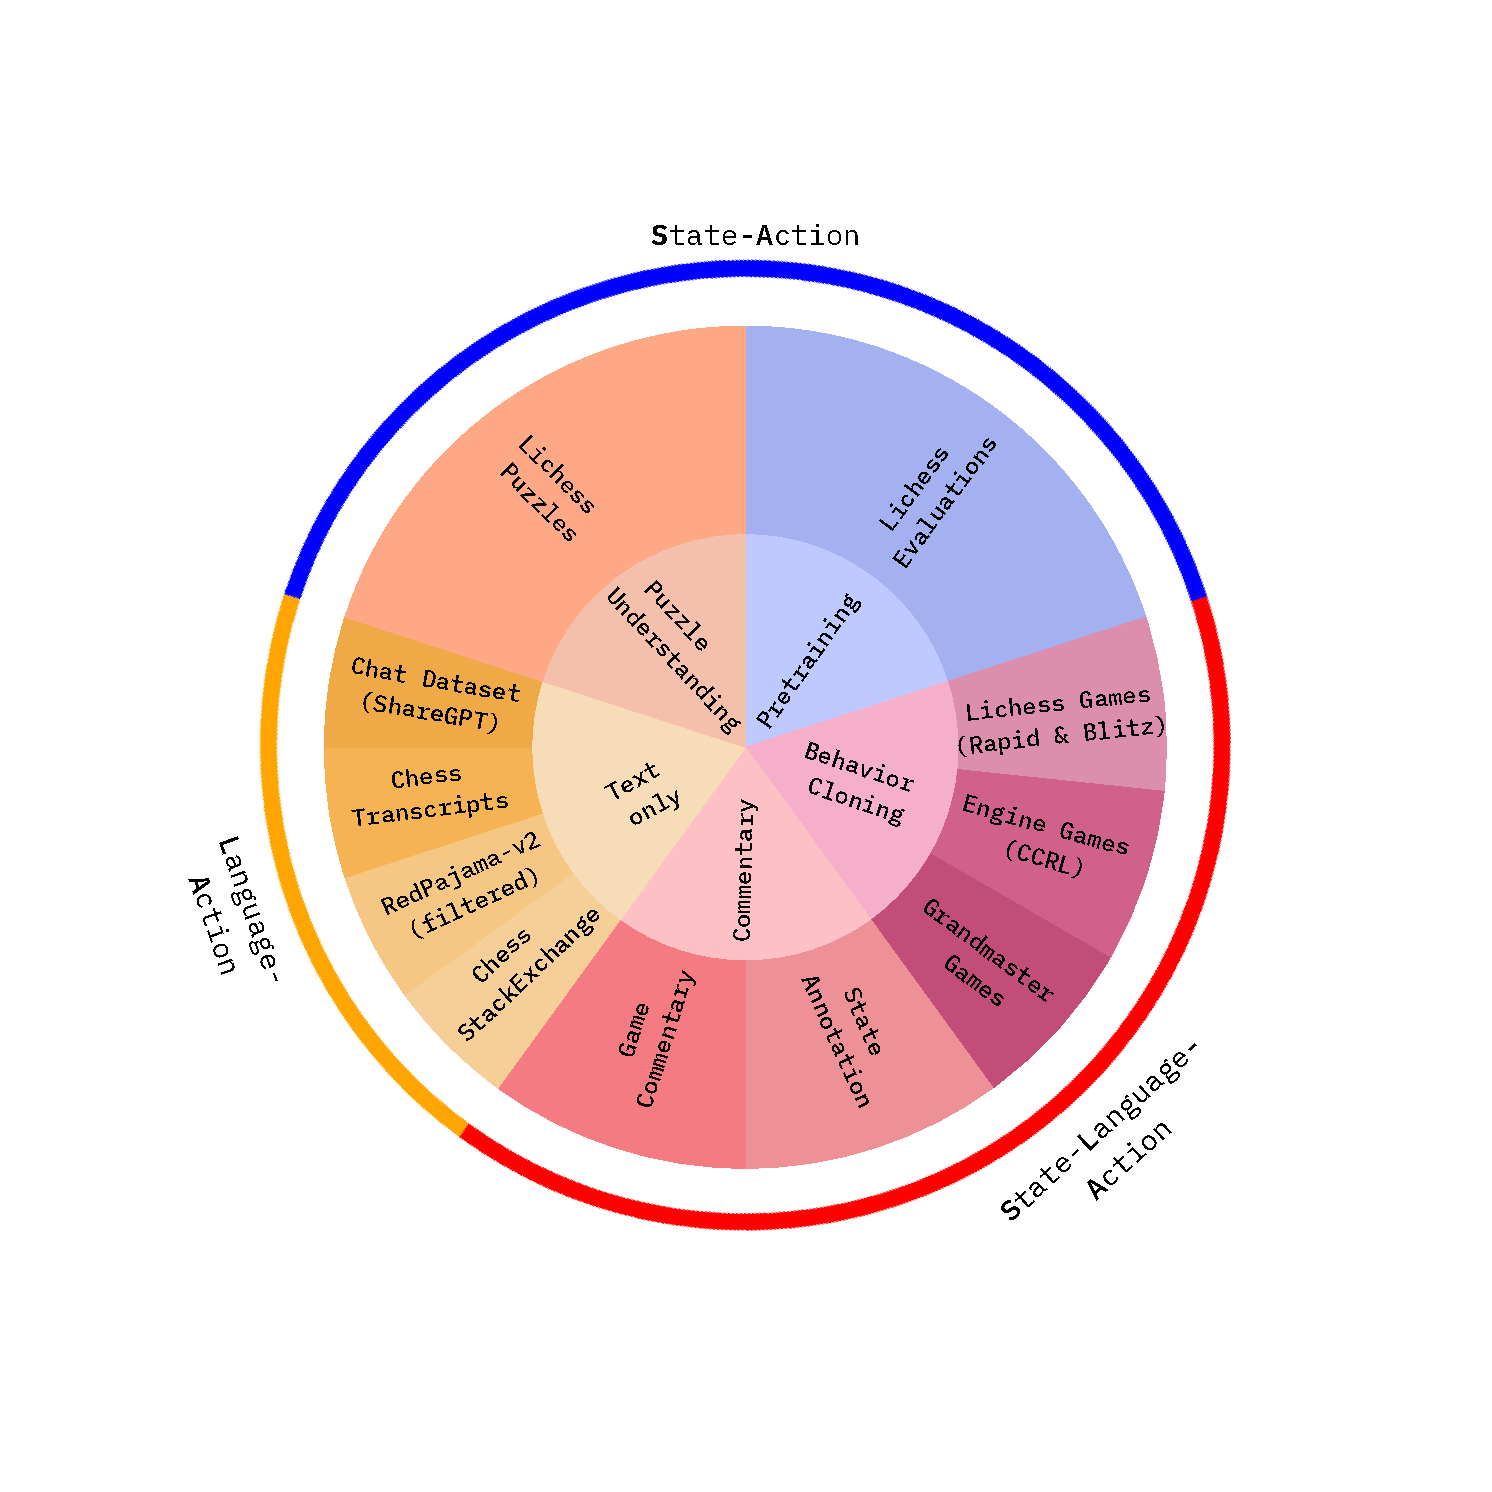
\includegraphics[width=0.98\linewidth]{data.pdf}
    \vspace{-8mm}
    \caption{The inner circle represents the distribution of training data, detailing the categories. The outer circle lists the types and data sources present in each category.}
    \label{fig:data}
\end{figure}

\begin{figure}[!h]
    \centering
    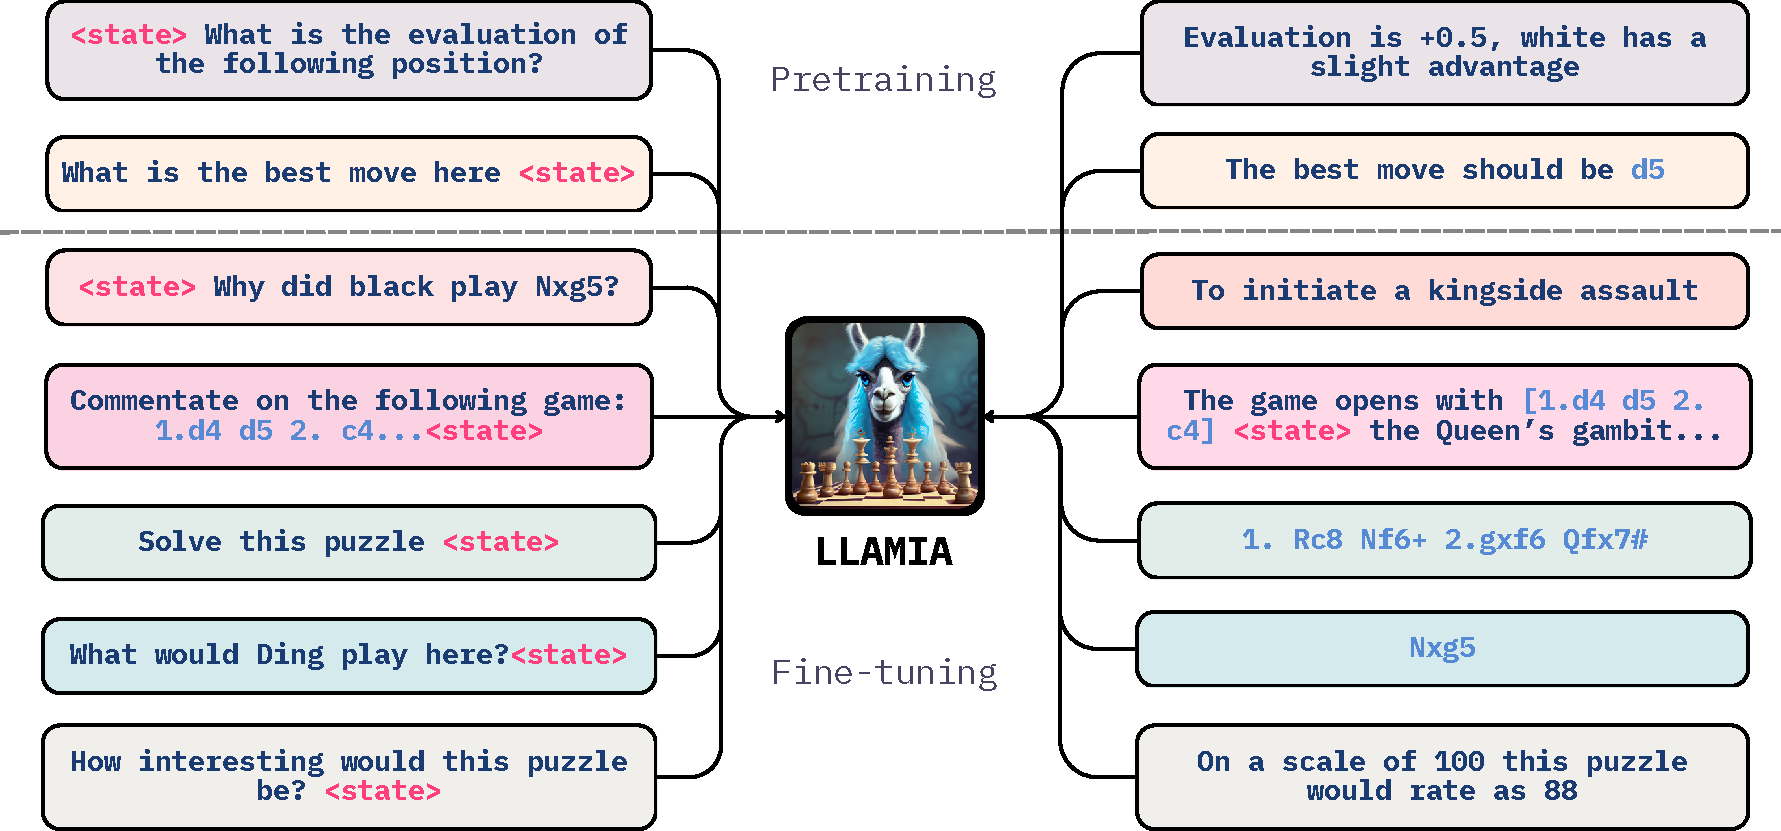
\includegraphics[width=0.98\linewidth]{llamia-tasks3.pdf}
    \caption{Tasks demonstrating LLAMIA capabilities across planning, reasoning, and acting: chess evaluations, best move predictions, behavior cloning, commentary prediction, state annotation, and puzzle understanding.}
    \label{fig:LLAMIA-arch-tasks}
\end{figure}

\subsubsection{Stage 1: Projector Alignment}
\label{sec:stage1}

We train only the projection network $H_\varphi$ to align the agent's latent representations $\vh_s$ with the LLM's token embedding space, while keeping the language model $\pi_\theta$ frozen. We construct a large-scale dataset $\mathcal{D}_{\text{pre}} = \{(s, \pi(s))\}$ by sampling state-policy pairs from the pretrained agent's self-play. Each example is paired with a language prompt (e.g., ``Analyze position: top move?''), and the model learns to generate the correct action token corresponding to $\pi(s)$. The exact prompt format is given in Listing~\ref{listing:pretraining_instruction_format}. Training minimizes the cross-entropy loss:
\[
\mathcal{L}_{\text{Stage\,1}} = -\mathbb{E}_{(s, \pi(s)) \sim \mathcal{D}_{\text{pre}}} \log \pi_\theta\!\left( \pi(s) \mid \vz_s, \text{prompt} \right)
\]
Because the LLM is frozen, the projector can be trained on abundant agent-generated data without risking catastrophic interference with language modeling.

\subsubsection{Stage 2: Reinforcement Learning}
\label{sec:stage2}

The second stage unfreezes both the LLM $\pi_\theta$ and the projector $H_\varphi$, and optimizes them jointly via DAPO~\cite{XXXdapo}. Rollouts produce complete mixed-modality traces $\tau$ (Eq.~\ref{eq:trace}); the policy gradient operates over positions where the LLM generates---\mlang{language} and \maction{action} tokens---while \mstate{state} positions are agent-injected and excluded from the gradient:
%
\begin{equation}
J(\theta, \varphi) \!=\! \mathbb{E}_{\tau \sim \pi_{\theta_{\mathrm{old}}}} \!\Bigg[\!
  \frac{1}{|\mathcal{I}_{\mathrm{gen}}|}
  \!\!\sum_{t \,\in\, \mlang{\mathcal{I}_{L}} \,\cup\, \maction{\mathcal{I}_{A}}}
  \!\!\min\!\Big(
    r_t\,\hat{A}_t,\,
    \mathrm{clip}(r_t, 1\!-\!\varepsilon_l, 1\!+\!\varepsilon_h)\,\hat{A}_t
  \Big)
\Bigg]
\label{eq:dapo}
\end{equation}
%
where $\hat{A}_t$ is the group-normalized advantage and the asymmetric clip bounds $\varepsilon_l \leq \varepsilon_h$ encourage exploration~\cite{XXXdapo}. The reward decomposes as $\mathcal{R}(\tau) = R_{\mathrm{outcome}} + R_{\mathrm{format}} + R_{\mathrm{collab}}$, combining task performance, syntactic validity, and a collaboration-shaping signal; full definitions are given in Appendix~\ref{sec:app_reward}.

Because the projector $H_\varphi$ is now unfrozen, the RL objective optimizes the integration interface end-to-end: gradients flow from the reward through the LLM's generated tokens back to the projector, shaping \emph{how} the agent's latent state is presented to the LLM---not just how the LLM uses it.

\subsubsection{Agent Invocation}
\label{sec:invocation}

LLAMIA invokes the agent through a structured tool call that the LLM learns to emit during RL. The call specifies a state---either the current environment state or a counterfactual state reached by a hypothetical action---and the agent encodes the specified state via $G_\psi$. The projector maps the result to $k$ latent tokens via $H_\varphi$, which are inserted into the trace, after which the LLM resumes autoregressive generation.

This mechanism creates a closed loop: the LLM reasons in language, acts on the environment, and queries the agent for a fresh encoding of the resulting state. Crucially, RL optimizes not only what the LLM does with the agent's response but also \emph{when} and \emph{whether} it invokes the agent---the invocation itself is part of the policy's action space. We show in \S\ref{sec:experiments} that removing dynamic re-encoding degrades multi-step tasks by 64\% while leaving single-step perception tasks largely unaffected (1--4\%), confirming that learned invocation timing is essential for sustained collaboration.

\section{Experiments and Results}
\label{sec:experiments}

We evaluate \textsc{LLAMIA} on \textsc{LLAMIA-Bench}, a suite of six tasks spanning three collaboration facets: behavioral imitation, state assessment, and natural-language explanation (\cref{sec:app_bench}). For comparing LLAMIA with closed source models where training isnt possible, we pair them with Lc0 as a verbalized tool. To evaluate against open-source models we create three settings: an untrained tool-use baseline, a 
training-matched verbalization system, and our internalized model, isolating the integration interface as the sole variable.  Within the 
open-source trained systems, we report both SFT and SFT + DAPO checkpoints to disentangle the contributions of supervised pretraining and reinforcement 
learning.
\somesh{add what conclusions are we showing}




\subsection{LLAMIA-Bench}
\textsc{LLAMIA-Bench} spans six tasks drawn from prominent problems in chess literature and industry, each unsolvable by either component alone: the subagent produces no language, while the LLM lacks the positional signals that make chess-specific judgments possible. The suite covers behavior cloning, puzzle understanding, move annotation, and game-level commentary (details in \cref{sec:app_bench}).
  Behavior cloning, difficulty estimation, and move annotation are drawn from established benchmarks~\cite{mcilroy2020aligning,lichess2024puzzles,jhamtani-etal-2018-learning}. We introduce three new evaluation targets: \textbf{Wild BC}, three OOD
  splits (GM-25, Low-Time, $\Delta$Elo) probing generalization to grandmaster play, time pressure, and asymmetric skill-gap
  ; \textbf{interest estimation}, ranking puzzles by community-derived interestingness scores, a signal with no
   verbal proxy in any engine output; and \textbf{Agadmator-2K}, the first large-scale game-level commentary dataset of 1,900 narrated games with move-aligned
  transcripts.
  Full dataset descriptions, metrics, and per-task prompts appear in Appendices~\ref{sec:app_bench}--\ref{sec:app_prompts}.
\subsection{Setup}
\label{sec:exp_setup}


\paragraph{Baselines}
We compare four systems. \textbf{(1) GPT-5.1\,+\,Lc0}: the strongest frontier model with verbalized Lc0-BT4 tool access. \textbf{(2) Qwen3-14B\,+\,Lc0}: the LLAMIA backbone with the same verbalized tool and 5-shot prompting, without training. \textbf{(3) LLAMIA-Verb}: the matched-recipe ablation with the latent channel replaced by the verbalized tool, isolating the integration interface as the sole variable. \textbf{(4) LLAMIA}: our full system with latent state-token integration. Extended comparisons including LLM-only baselines, SFT and DAPO checkpoints at all three model sizes(4B,8B and 14B), frontier model comparisons, and task-specific experts are in \cref{sec:app_results}. Training details and hyperparameters are in Appendix~\ref{sec:app_implementation}.

\paragraph{Metrics}
Each task has a primary metric detailed in \cref{sec:app_bench}: move-matching accuracy (behavior cloning), Spearman $\rho$ (difficulty and interest), and G-eval and BLEU-2 (annotation and commentary). Primary metrics include 95\% bootstrap confidence intervals where sample sizes warrant; per-task breakdowns with CIs appear in \cref{sec:app_results}.

\subsection{Main Results}
\label{sec:results_main}
\somesh{The key results seem mixed/missing here, we have to compare LLAMIA outperforms top frontier LLMs which are much larger and existing state of the art methods with 14B, referring to table 1 and competitive with 8B, 4B etc referring to table full\_bench  mentioning we remain close to Allie while being significantly better in Wild BC. Next, mention the extensive evaluation including more metrics, baselines, for each task paired with reference to those tables. Another heading should be that LLAMIA unlocks new tasks (Interest) where all other methods have almost 0 performance}
\begin{figure*}[t]
    \centering
    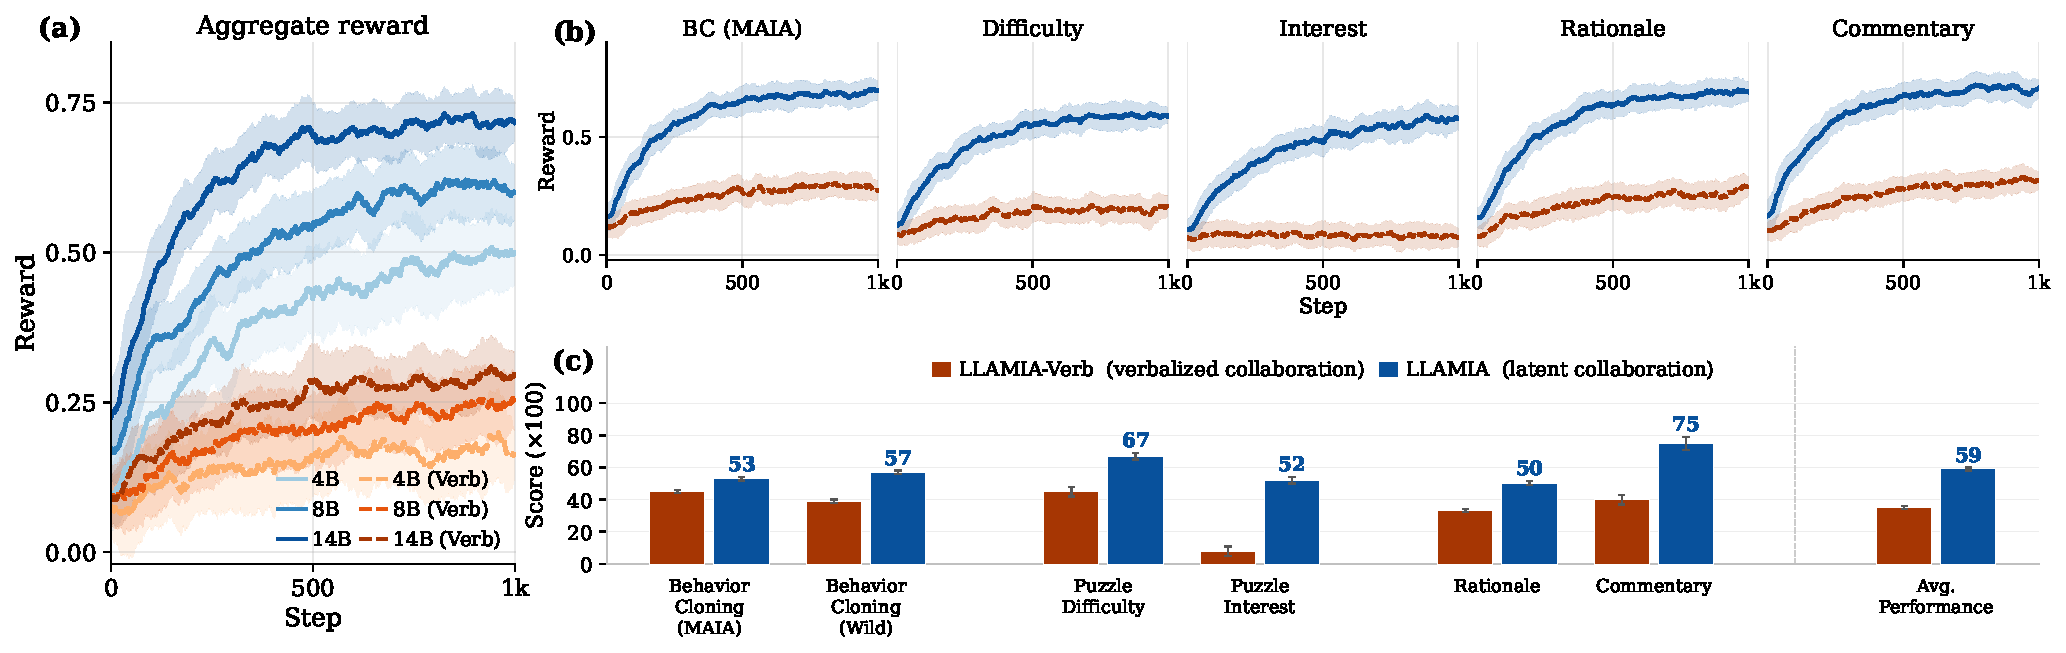
\includegraphics[width=\linewidth]{plots/combined_training_bench_verb_vs_llamia.pdf}
    \caption{%
    \textbf{DAPO training dynamics and LLAMIA-Bench evaluation.}
    \textbf{(a)}~Aggregate reward vs.\ training step at three backbone scales.
    Solid: LLAMIA (latent); dashed: LLAMIA-Verb (verbalized, identical recipe and backbone).
    The debt widens throughout and reaches $2$--$3\times$ by convergence; scaling the backbone does not close it for LLAMIA-Verb.
    \textbf{(b)}~Per-task reward curves at 14B.
    LLAMIA-Verb gains partial signal on behavior cloning and difficulty (tasks with verbalizable proxies) but stays near-flat on interest and commentary, where the reward requires non-verbalizable features or multi-step integration.
    \textbf{(c)}~LLAMIA-Bench scores ($0$--$100$).
    Puzzle Interest is diagnostic: every verbalized system scores ${\leq}12$ regardless of model scale or frontier capability, while LLAMIA-14B reaches $52$.
    Full per-task tables with confidence intervals in \cref{sec:app_results}.
    }
    \label{fig:combined}
\end{figure*}
LLAMIA-14B achieves the highest score on all six \textsc{LLAMIA-Bench} tasks (\cref{fig:combined}c), surpassing frontier verbalized systems an order of magnitude larger and remaining competitive with dedicated task-specific finetunes that are trained on substantially more in-domain data.
On behavior cloning, Maia and Allie are trained on tens of millions of chess-specific games, against LLAMIA's general-purpose backbone. LLAMIA-14B remains inside the expert band on the in-distribution Maia split and surpasses the strongest expert by a wide margin on the OOD Wild splits (GM-25, Low-Time, $\Delta$Elo), which probe regimes absent from the experts' blitz-only training mixture. Latent access to the engine's policy and value structure thus generalizes more reliably than direct supervision on a narrower distribution. Interest and commentary have no dedicated task-specific baseline at all, no published system predicts puzzle interestingness or generates grounded move commentary from engine state, which is itself evidence that these tasks require the joint reasoning LLAMIA provides rather than a narrower specialist.
The advantage over GPT-5\,+\,Lc0 does not require the 14B backbone: LLAMIA-8B already leads on all six tasks, and LLAMIA-4B on four of six (\cref{tab:full_bench}).
Per-task evaluations with additional metrics, baselines, and confidence intervals are in \cref{sec:app_results}.

\paragraph{Latent tokens enable new evaluation targets.}
Puzzle Interest requires ranking positions by community-derived interestingness, a signal that depends on the engine's policy distribution and value gradients across candidate moves.
No verbalized engine output carries these features.
Every verbalized system scores ${\leq}12$ on Interest regardless of model scale or frontier capability; LLAMIA-14B reaches $52$ (\cref{fig:combined}c).
Verbalization has zero useful signal for this task, while latent tokens give the LLM direct access to the distributional structure that defines interestingness.


% \begin{table}[t]
% \centering
% \caption{\textbf{LLAMIA-Bench summary and verbalization debt.}
% All scores normalized $0$--$100$; higher is better. LLAMIA and LLAMIA-Verb share the same 14B backbone, Lc0-BT4 subagent, and DAPO recipe; the only difference is the integration interface (latent tokens vs.\ verbalized text). The $\Delta$ row reports the \textbf{verbalization debt} per task. Task-specific expert is the strongest published baseline per task (Allie-Adaptive-Search for BC, SCC for Annotation); blanks indicate no dedicated baseline. Full per-scale factorial in \cref{tab:full_bench}.}
% \label{tab:main_bench}
% \begin{adjustbox}{max width=\columnwidth}
% \begin{tabular}{l|cc|cc|c|c}
% \toprule[1.2pt]
% \textbf{System} &
% \multicolumn{2}{c|}{\textbf{BC}} &
% \multicolumn{2}{c|}{\textbf{Puzzle}} &
% \textbf{Ann.} &
% \textbf{Comm.} \\
% & \textbf{MAIA} & \textbf{Wild} &
% \textbf{Diff.} & \textbf{Int.} & & \\
% \midrule
% Task-Spec. Expert  & \valbest{55} & 45 & -- & -- & 34.5 & -- \\
% GPT-5+Lc0         & 45 & 40 & 48 & 10 & 37.5 & 55 \\
% LLAMIA-Verb-14B   & 45 & 39 & 45 & 8 & 33.2 & 40 \\
% LLAMIA-14B        & 53 & \valbest{57} & \valbest{67} & \valbest{52} & \valbest{50.3} & \valbest{75} \\
% \midrule
% $\Delta$ (debt)   & $+8$ & $+18$ & $+22$ & $+44$ & $+17.1$ & $+35$ \\
% \bottomrule[1.2pt]
% \end{tabular}
% \end{adjustbox}
% \end{table}
% =========================================================================
\subsection{Verbalization Debt}
\label{sec:results_vd}
\somesh{Now that we have quantitatively differentiated LLAMIA on all tasks against Frontier + Task specific Finetunes we discuss the verbalization debt through key headings, first, define it. Summarize the results from table 1, then from figure Verbalization debt is consistent across scale, and throughout training, from training dynamics figure.}

LLAMIA and LLAMIA-Verb share the same 14B backbone, Lc0-BT4 subagent, and DAPO recipe; the only difference is whether the subagent's state reaches the LLM as latent tokens or as verbalized text. We define the resulting performance gap as the \textbf{verbalization debt}.

\paragraph{Verbalization debt is significant across all tasks}
Figure \ref{fig:combined} shows that the verbalization debt is consistent across all six tasks. The gap is largest on Interest and Commentary, where the target signal lives in the engine's full policy distribution or value landscape and has no faithful text equivalent, and smallest on in-distribution behavior cloning, where the engine's top-$k$ moves already approximate the answer and the verbal summary loses little.

\paragraph{The debt persists across backbone scale.}
Increasing the LLM from 4B to 14B improves both systems, but the debt persists at every scale (\cref{tab:full_bench}). On Interest, LLAMIA-Verb-14B scores $8$ while LLAMIA-4B already reaches $38$.

\paragraph{The debt widens throughout training.}
The debt grows throughout DAPO, reaching $2$--$3\times$ by the end of training (\cref{fig:combined}a). Per-task reward curves (\cref{fig:combined}b) reveal where the verbal channel saturates: LLAMIA-Verb gains partial signal on behavior cloning and difficulty, where the verbalized output carries a useful proxy (top-$k$ moves, solution length), but stays near-flat on interest and commentary, where no such proxy exists.

\subsection{Ablations}
\label{sec:results_ablations}
To further understand the verbalization debt and isolate the contribution of internalization and reinforcement learning we conduct the following ablations and compare in \cref{tab:ablation_main}. \textbf{LLM-Only} trains with RL but no engine, so any gain has to come from the weights. \textbf{LLM-ChessCLIP} trains with RL and the same $32$ latent slots as LLAMIA, but filled by a raw board encoder (ChessCLIP, a PaLM-E-style injection) rather than Lc0's state, so any gain has to come from capacity rather than content. \textbf{Qwen3+Lc0 (untr.)} is untrained tool use. \textbf{LLAMIA-Verb} is RL on top of verbalized text. \textbf{LLAMIA-SFT (latent)} removes RL, the reasoning trace, and the invocation policy, leaving only the latent channel. \textbf{LLAMIA} is the full system. Extended controls, latent-only, shuffled tokens, per-task probes, and templates, are in \cref{sec:abl_interface,sec:app_baselines_probe}.

\begin{table}[t]
\centering
\caption{\textbf{Interface controls} (14B). BC in \% move-match; Difficulty and Interest in Spearman $\rho$; Rationale in BLEU-2; Commentary in G-eval. All trained systems share backbone, data, and recipe; only the interface differs.}
\label{tab:ablation_main}
\begin{adjustbox}{max width=\columnwidth}
\renewcommand{\arraystretch}{1.15}
\small
\begin{tabular}{lcccccc}
\toprule[1.2pt]
\textbf{System} & \textbf{BC-M} & \textbf{BC-W} & \textbf{Diff.} & \textbf{Int.} & \textbf{Rat.} & \textbf{Comm.} \\
\midrule
LLM-Only (RL, no engine)          & $34$ & $19$ & $0.22$ & $0.07$ & $16.1$ & $0.13$ \\
LLM-ChessCLIP (RL, raw encoder)   & $39$ & $28$ & $0.24$ & $0.08$ & $23.1$ & $0.29$ \\
Qwen3\,+\,Lc0 (untr.\ tool use)   & $39$ & $33$ & $0.28$ & $0.05$ & $18.8$ & $0.15$ \\
LLAMIA-Verb (RL, text only)       & $45$ & $39$ & $0.45$ & $0.08$ & $33.2$ & $0.40$ \\
LLAMIA-SFT (latent, no RL)        & $51$ & $46$ & $0.66$ & $0.48$ & $38.5$ & $0.58$ \\
LLAMIA (latent, RL)               & \valbest{$53$} & \valbest{$49$} & \valbest{$0.71$} & \valbest{$0.52$} & \valbest{$45.8$} & \valbest{$0.75$} \\
\bottomrule[1.2pt]
\end{tabular}
\end{adjustbox}
\vspace{-3mm}
\end{table}

\paragraph{The gain comes from Lc0's latent state, not from weights or capacity.}
LLM-Only and LLM-ChessCLIP get the same RL recipe as LLAMIA and still land near or below untrained tool use, so DAPO cannot manufacture the missing expertise on its own, whether it is asked to bake it into the weights or to make sense of $32$ slots filled with the wrong content. Shuffling LLAMIA's own latent tokens produces the same collapse toward LLAMIA-Verb even though the token count never changes (\cref{sec:abl_interface}). The pattern only breaks when those slots carry Lc0's own policy and value representations. Further, LLAMIA-SFT, with no RL recovers most of the verbalization debt. However, it compounds the effect of internalization by bringing the improvements in multi step strategies, where the model has to plan across latent states i.e. Game Commentary and Rationale generation. We further show this through the emergent latent collaboration strategies in \cref{sec:results_agency}.

\subsection{Collaboration Strategies}
\label{sec:results_agency}
\somesh{The signposting or motivation of why we are discussing Collaboration strategies is missing. `apart from quantitative comparison in agent performance we now analyze the learnt collaboration strategies through internalization and RL over multi-step planning. We qualitatively analyze and identify the following dominant patterns of subagent invokation and actions as shown in figure 2. We describe these patterns and their definitions in appendix ... Then key headlines, training for strategic collaboration with non language agent collapses with verbalization, whereas with internalization LLAMIA exhibits better agency with task specific strategies learnt during training. Defer to dynamics from figure only.}
Does the integration interface determine how the model learns to use the subagent, or only how well it performs? We classify subagent invocations during evaluation into five recurring strategies and trace their evolution during DAPO training (\cref{fig:agency_task_specificity}; strategy definitions and per-task heatmaps in \cref{fig:agency_heatmaps}).

\begin{figure}[t]
    \centering
    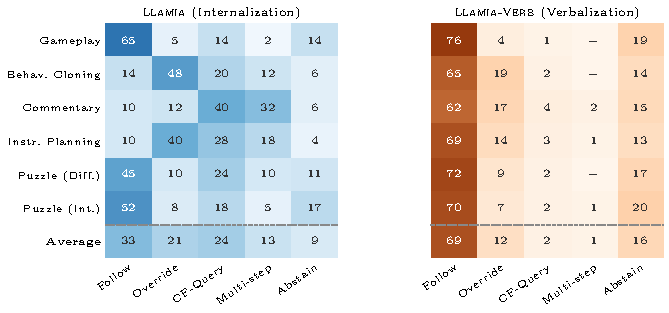
\includegraphics[width=\linewidth]{pages/figures/agency_strategy_heatmaps.pdf}
    \caption{\textbf{Collaboration strategy distribution (\%) per task at convergence.}
  Fraction of 500 episodes assigned to each strategy by a GPT-4o judge
  ($\kappa{=}0.78$). \emph{Left:} LLAMIA (latent). \emph{Right:} LLAMIA-Verb
  (verbalized). LLAMIA's dominant strategy shifts with the task
  (engine-follow for gameplay, consult-then-override for BC, counterfactual
  query for commentary); LLAMIA-Verb collapses to engine-follow on every
  row (62--76\%). Detailed discussion can be found in \cref{sec:abl_agency_strategies}}
    \label{fig:agency_heatmaps}

    \vspace{-2mm}
\end{figure}


The five strategies are \emph{engine-follow} (adopt the top recommendation), \emph{consult-then-override} (query then diverge), \emph{counterfactual query} (play a hypothetical move, re-invoke, compare states), \emph{multi-step lookahead} (chain two or three counterfactual sequences), and \emph{abstention} (act from language knowledge alone). A GPT-4o judge classifies 500 episodes per task per system ($\kappa{=}0.78$ vs.\ human raters).

\paragraph{Internalization produces task-specific collaboration; verbalization collapses it.}
LLAMIA adapts its strategy to the task: engine-follow dominates gameplay (65\%), consult-then-override dominates behavior cloning (48\%), and counterfactual query dominates commentary (40\%). LLAMIA-Verb collapses to engine-follow on every task (62--76\%), regardless of what the task requires (\cref{fig:agency_heatmaps}). The verbalized channel returns the same compressed summary no matter how the model queries it, so RL converges on a single use pattern.

\paragraph{The learned strategy makes internalization inference-cost neutral.}
Because it reasons over the full latent state, LLAMIA learns to invoke the subagent less often than LLAMIA-Verb ($1.9$ vs.\ $2.9$ calls per query at 14B). Each latent invocation adds a fixed $32$ tokens ($182$ vs.\ $150$), but the lower call count offsets this, so average tokens-per-query and wall-clock latency are comparable or lower than the verbalized interface; training cost stays within ${\sim}6\%$ of the verbalized pipeline at every scale (\cref{sec:app_cost}). Latent internalization therefore does not trade accuracy for inference cost.

\subsection{Human Evaluation}
\label{sec:results_human}

\begin{figure*}[t]
    \centering
    \begin{subfigure}[t]{0.235\linewidth}
        \centering
        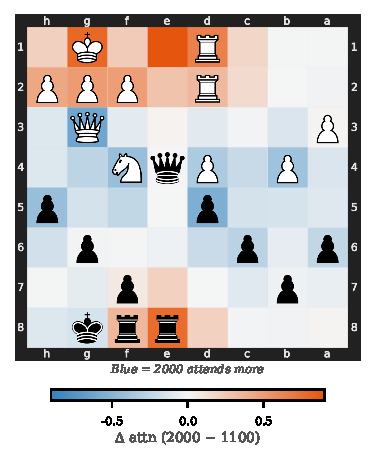
\includegraphics[width=\linewidth]{pages/figures/board_heatmap_c4_diff.pdf}
        \label{fig:human_heatmap}
    \end{subfigure}\hfill
    \begin{subfigure}[t]{0.245\linewidth}
        \centering
        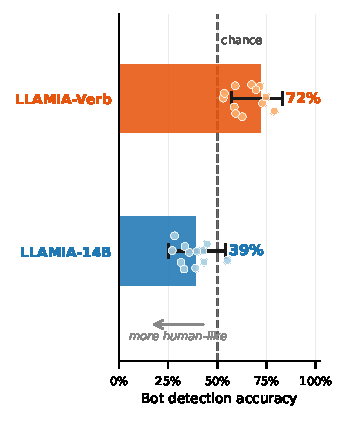
\includegraphics[width=\linewidth]{pages/figures/llamia_human_gameplay_compact.pdf}
        \label{fig:human_gameplay_main}
    \end{subfigure}\hfill
    \begin{subfigure}[t]{0.245\linewidth}
        \centering
        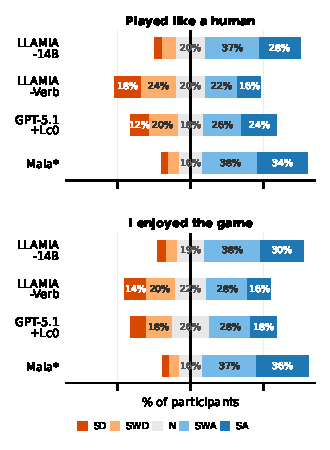
\includegraphics[width=\linewidth]{pages/figures/llamia_survey_vert.pdf}
        \label{fig:human_survey_main}
    \end{subfigure}\hfill
    \begin{subfigure}[t]{0.245\linewidth}
        \centering
        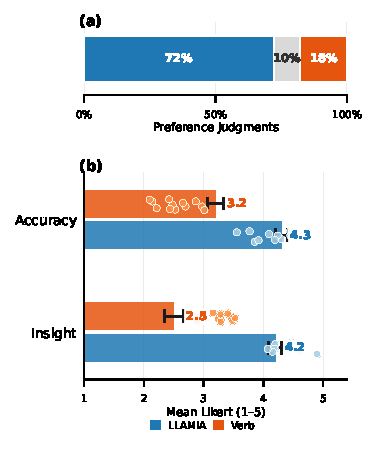
\includegraphics[width=\linewidth]{pages/figures/llamia_human_commentary_compact.pdf}
        \label{fig:human_commentary_main}
    \end{subfigure}
    \vspace{-4mm}
    \caption{%
    \textbf{Human evaluation ($n{=}12$ skilled players, all rated ${\geq}1700$).}
    \textbf{(a)}~Attention difference over latent tokens on a back-rank mate position: conditioning on 2000~Elo concentrates attention on mating geometry (red); 1100~Elo disperses to material (blue). The same latent state is read differently depending on the language instruction.
    \textbf{(b)}~Bot-detection rate (Study~1): LLAMIA-14B passes as human in 61\% of trials (detection 39\%, below chance); LLAMIA-Verb detected in 72\%.
    \textbf{(c)}~Post-game Likert (Strongly Disagree $\rightarrow$ Strongly Agree): LLAMIA matches Maia* (best Maia variant per Elo bucket) on human-likeness without training on human-move distributions.
    \textbf{(d)}~Commentary preference (Study~2): 72.2\% of 180 judgments favour LLAMIA; Insight gap (1.7\,pts) exceeds Accuracy gap (1.1\,pts).
    Study design and qualitative results in \cref{sec:app_human}.
    }
    \vspace{-3mm}
    \label{fig:human_eval}
\end{figure*}

\paragraph{Gameplay.}
Skilled players ($n{=}12$, all ${\geq}1700$ Elo) cannot reliably distinguish LLAMIA from a human opponent: detection falls below chance (\cref{fig:human_gameplay_main}), and post-game ratings place LLAMIA alongside Maia* on perceived human-likeness (\cref{fig:human_survey_main}). Maia is trained directly on millions of move distributions; LLAMIA receives no human-move supervision. Instead, behavioral signatures such as time-pressure blunders and skill-appropriate piece saliency emerge from latent-state conditioning alone. LLAMIA-Verb, trained with the same backbone and DAPO budget, is detected at rates well above chance, consistent with the stylistic regularities that verbal summaries impose on move selection.

\paragraph{Commentary.}
Both systems achieve comparable factual accuracy: material balance, initiative assessment, and basic evaluations survive verbalization reasonably well. The gap concentrates on strategic insight (\cref{fig:human_commentary_main}), where participants rate LLAMIA higher by a wider margin on the Insight dimension than on Accuracy. Text preserves \emph{what} is happening on the board, but explaining \emph{why} a move is strong requires representational features (policy gradients, value topology, look-ahead depth) that do not survive verbal compression.

\paragraph{Latent tokens are instruction-modulated.}
On a fixed back-rank mate position (\cref{fig:human_heatmap}), LLAMIA's attention over the latent tokens shifts with the target Elo: at 2000 it concentrates on the mating geometry, at 1100 it disperses to material. The latent representation is identical in both cases; what changes is the LLM's reading, conditioned on the natural-language Elo instruction. The projected state functions as a perceptual input shaped by task context, not a static feature vector.

\subsection{Generalization Beyond Chess}
\label{sec:results_go}

To provide initial evidence that LLAMIA can transfer beyond chess, we instantiate it on Go. We use KataGo-b18~\cite{wu2019katago}, a state-of-the-art Go neural engine, as the non-language subagent. We train a three-layer LatentBridge, with the first-layer width matched to KataGo's $384$ trunk channels and the $361$ board intersections represented as spatial tokens, using the same two-stage DAPO procedure on rank-conditioned behavior cloning. LLAMIA-Go-$14$B achieves $48$/$50$ top-1 human move-match at ranks 5k/5d using only $8$k positions, matching the rank-calibrated KataGo-HumanSL expert~\cite{wu2024katagohuman} and outperforming the verbalized control by ${\sim}10$ points. The latent-over-verbal gap remains consistent across the 4B, 8B, and 14B model scales (\cref{sec:app_go}). These results provide strong evidence that latent collaboration is not specific to chess. Establishing broader generality across environments and task families remains an important direction for future work.
\section{Related Work}
\vspace{-2mm}
The dominant paradigm for LLM-agent integration is text-mediated: ReAct~\cite{yao2022react}, Toolformer~\cite{schick2023toolformerlanguagemodelsteach}, and multi-agent orchestrators like AutoGen~\cite{wu2023autogen} and HuggingGPT~\cite{shen2024hugginggpt} all route communication through natural language. This is lossless when both parties are language models, but compresses the policy and value representations of pretrained neural agents into a few tokens. A parallel line moves reasoning itself into continuous representations to escape the bandwidth limit of discrete tokens~\cite{zhu2025surveylatentreasoning}, either through latent recurrence within one model (CoCoNut~\cite{hao2025traininglargelanguagemodels}) or by interleaving latent and text tokens in a single reasoning stream (Token Assorted~\cite{su2025tokenassorted}, latent tokens as extra computation~\cite{sun2025latenttokens}); these operate on a model's \emph{own} hidden state, not a separate agent's. Latent channels exist in multi-agent RL~\cite{sukhbaatar2016learningmultiagentcommunicationbackpropagation,das2019tarmac,foerster2016learning} and homogeneous LLMs~\cite{latentmas2025}, but assume jointly trained or homogeneous populations, not a frozen LLM with a frozen specialist. Cross-modal injection (PaLM-E~\cite{driess2023palmeembodiedmultimodallanguage}, RT-2~\cite{brohan2023rt2visionlanguageactionmodelstransfer}) projects raw sensory observations, not a pretrained agent's processed policy/value representations. None of these internalizes a non-language specialist's latent state into an LLM (\cref{tab:related_distinction}). On the domain side, neural chess engines encode rich positional structure in their activations~\cite{silver2017mastering,monroe2024mastering}, as interpretability work confirms~\cite{jenner2024evidence}, yet prior LLM-chess work either trains task-specific models~\cite{jhamtani-etal-2018-learning} or conditions on verbalized outputs~\cite{feng2024chessgpt}; none exposes the engine's latent state to the LLM.

\vspace{-3mm}
\section{Conclusion}
\label{sec:conclusion}
\vspace{-3mm}
We introduced latent state internalization, an LLM--agent integration method that
replaces verbalized communication with direct projection of an agent's continuous
representations into the LLM's embedding space. LLAMIA-14B, trained via
projector alignment followed by DAPO, matches or exceeds dedicated task finetunes across
\textsc{LLAMIA-Bench}. The verbalization debt widens with interaction depth and on
signals that resist text serialization (e.g., puzzle interest), and does not close with LLM scale or RL budget in
our evaluated range, indicating verbalization is a structural bottleneck for LLM--agent
collaboration.



\bibliographystyle{iclr2026_conference}
\bibliography{sample}

\clearpage
\appendix

\startcontents[appendices]
\printcontents[appendices]{}{1}{}
\clearpage

% --------------- Appendix setup -----------------------------------------------
% Allow page breaks after headings even when no content follows yet (skeleton).
% Standard LaTeX sets \@nobreaktrue after every heading, preventing page breaks
% until real content appears. With an empty skeleton this causes overflow.
% We force \@nobreakfalse so LaTeX can break between consecutive headings.
\makeatletter
\def\@afterheading{%
  \@nobreakfalse
  \everypar{%
    \if@nobreak
      \@nobreakfalse
      \clubpenalty \@M
      \if@afterindent \else
        {\setbox\z@\lastbox}%
      \fi
    \else
      \clubpenalty \@clubpenalty
      \everypar{}%
    \fi}}
\makeatother

% --------------- Appendix TOC ------------------------------------------------
\etocsettocdepth.toc{subsubsection}% from here on, write section/subsection/subsubsection to .toc

\section*{Appendix Table of Contents}
\label{sec:appendix_toc}

\begingroup
\small
\setlength{\parskip}{0pt}%
\etocsetnexttocdepth{subsubsection}%
\etocsettocstyle{}{}%
\etocsetstyle{section}%
  {}% global prefix
  {\vspace{3pt}}% prefix
  {\noindent\bfseries\makebox[1.8em][l]{\etocnumber}\etocname\dotfill\,\etocpage\par}%
  {}%
\etocsetstyle{subsection}%
  {}{}%
  {\noindent\hspace{1.8em}\makebox[2.4em][l]{\etocnumber}\etocname\dotfill\,\etocpage\par}%
  {}%
\etocsetstyle{subsubsection}%
  {}{}%
  {\noindent\hspace{4.2em}\makebox[2.8em][l]{\etocnumber}\etocname\dotfill\,\etocpage\par}%
  {}%
\tableofcontents
\endgroup

\vspace{1em}
\hrule
\vspace{1em}

% --------------- Sections ----------------------------------------------------

% =============================================================================
\section{Implementation Details}
\label{sec:app_implementation}
% =============================================================================

\subsection{Model Architecture and LatentBridge}
\label{sec:app_architecture}

\subsubsection{Backbone LLM}
\label{sec:app_backbone}

\subsubsection{LatentBridge Projector}
\label{sec:app_projector}

\subsection{Training Configuration}
\label{sec:app_training}

\subsubsection{Stage 1: Projector Alignment}
\label{sec:app_stage1}

\subsubsection{Stage 2: Reinforcement Learning (DAPO)}
\label{sec:app_stage2}

\subsection{Chess Specialist: Lc0-BT4}
\label{sec:app_lc0}

\subsubsection{Engine Configuration}
\label{sec:app_lc0_config}

\subsubsection{Latent Extraction}
\label{sec:app_lc0_latent}

\subsection{Inference Harness and Tool-Call Protocol}
\label{sec:app_toolcall}

\subsubsection{Agent State}
\label{sec:app_toolcall_state}

\subsubsection{System Prompt}
\label{sec:app_toolcall_prompt}

\subsubsection{Tool Definitions}
\label{sec:app_toolcall_tools}

\subsection{Training Efficiency (FSDP)}
\label{sec:app_efficiency}

% =============================================================================
\section{LLAMIA-Bench}
\label{sec:app_bench}
% =============================================================================

% Shared macros for this section
\providecommand{\tbd}{\textcolor{gray}{\texttt{[TBD]}}}
\providecommand{\itwmark}{\textsuperscript{$\star$}}

% Per-task-group row colours (xcolor)
\definecolor{clrGameplay}{RGB}{215,230,255}
\definecolor{clrBC}{RGB}{210,245,210}
\definecolor{clrStylo}{RGB}{238,218,255}
\definecolor{clrPuzzle}{RGB}{255,245,200}
\definecolor{clrAnnot}{RGB}{205,245,245}
\definecolor{clrComm}{RGB}{255,218,232}
\definecolor{clrICP}{RGB}{228,228,228}

% =============================================================================
\subsection{Dataset}
\label{sec:app_bench_dataset}
% =============================================================================

LLAMIA-Bench evaluates LLM--specialist-agent collaboration across six facets: \emph{perception}, \emph{calibration}, \emph{explanation}, \emph{sustained planning}, \emph{style and identity}, and \emph{instruction-conditioned adaptation}. Each task carries externally verifiable ground truth and shares a uniform input--output surface across integration regimes (text-only, verbalized-tool, latent-internalized), so the Verbalization Gap and Depth-Compounding Slope emerge as corollaries from a single suite. Table~\ref{tab:bench_dataset} summarizes dataset sources, train/test sizes, evaluation metrics, prior task experts, and RL reward signals. Splits marked~\itwmark{} are \emph{in-the-wild}: the test distribution is sparse, absent, or shifted relative to the Stage-2 training corpus and generalization must come from internalized representations.

\begin{table*}[ht]
\centering
\caption{%
  \textbf{LLAMIA-Bench dataset and task summary.}
  \textbf{Task / Split}: evaluation unit (LLAMIA-Bench custom splits in \emph{italics}).
  \textbf{Dataset}: canonical name used in this paper.
  \textbf{Source}: data origin.
  \textbf{Size}: train\,/\,held-out test.
  \textbf{Metrics}: primary evaluation metric(s); $\uparrow$ higher is better, $\downarrow$ lower is better.
  \textbf{Task Expert}: strongest prior specialist baseline on this task.
  \textbf{RL Reward}: outcome reward signal for DAPO Stage~2.
  \itwmark{}\,=\,in-the-wild split.
  \tbd\,=\,to be finalized.
}
\label{tab:bench_dataset}
\setlength{\tabcolsep}{4pt}
\begin{adjustbox}{max width=\textwidth}
\renewcommand{\arraystretch}{1.35}
\small
\begin{tabular}{p{2.4cm} p{2.1cm} p{2.3cm} p{2.1cm} p{3.0cm} p{2.5cm} p{3.0cm}}
\toprule[1.2pt]
\textbf{Task / Split} & \textbf{Dataset} & \textbf{Source} & \textbf{Size (train\,/\,test)} & \textbf{Metrics} & \textbf{Task Expert} & \textbf{RL Reward} \\
\midrule

%% ── GAMEPLAY ─────────────────────────────────────────────────────────────────
\multicolumn{7}{@{\hspace{2pt}}l}{\cellcolor{clrGameplay}\textbf{Gameplay}} \\[-3pt]
\rowcolor{clrGameplay}
Elo Rating
  & Tournament Elo
  & ECO openings; BayesElo~\cite{coulom2008whole}
  & --\,/\,1k games/pair
  & Tournament Elo $\pm$CI $\uparrow$
  & Transformer-270M~\cite{ruoss2024grandmaster}
  & Game outcome ($+1$ win, $0$ draw, $-1$ loss) \\
\rowcolor{clrGameplay}
Puzzle Solving
  & Lichess Puzzles
  & \texttt{lichess.org}
  & 4M\,/\,1K
  & Exact-sequence Acc.\ (\%) $\uparrow$
  & Transformer-270M~\cite{ruoss2024grandmaster}
  & $+1$ iff full solution sequence correct, else $0$ \\

%% ── BEHAVIOR CLONING ─────────────────────────────────────────────────────────
\midrule
\multicolumn{7}{@{\hspace{2pt}}l}{\cellcolor{clrBC}\textbf{Behavior Cloning}} \\[-3pt]
\rowcolor{clrBC}
Maia (Elo Buckets)
  & MAIA-KDD
  & Lichess~\cite{mcilroy2020aligning}
  & 12M\,/\,MAIA test set
  & Move-match Acc.\ per bucket $\uparrow$
  & Maia-1900; Maia+MCTS~\cite{jacob2022modeling}
  & Move-match with target-Elo policy \\
\rowcolor{clrBC}
\emph{GM-25}\,\itwmark{}
  & GM-25
  & 365chess.com; FIDE top-25 historical
  & $\leq$4,641 games/GM\,/\,--
  & Move-match Acc.\ $\uparrow$
  & Per-GM Maia model
  & Move-match with GM-specific corpus \\
\rowcolor{clrBC}
\emph{Low-Time}\,\itwmark{}
  & Low-Time BC
  & Lichess (time-pressure flag)
  & 129K pos.\,/\,--
  & Move-match Acc.\ $\uparrow$
  & Maia (matched Elo)
  & Move-match under clock pressure \\
\rowcolor{clrBC}
\emph{Elo Gap}\,\itwmark{}
  & Elo-Gap BC
  & Lichess ($\Delta$Elo $>$ 500)
  & 34K games\,/\,--
  & Move-match Acc.\ $\uparrow$
  & Maia (matched Elo)
  & Move-match in large skill-gap games \\

%% ── BEHAVIORAL STYLOMETRY ────────────────────────────────────────────────────
\midrule
\multicolumn{7}{@{\hspace{2pt}}l}{\cellcolor{clrStylo}\textbf{Behavioral Stylometry}} \\[-3pt]
\rowcolor{clrStylo}
\emph{GM Identification}\,\itwmark{}
  & GM-Stylo
  & Held-out GM game corpus
  & \tbd\,/\,\tbd
  & Top-1/2/3 identification Acc.; Bradley--Terry ranking~\cite{CvjXlsBLCX-strength-est} $\uparrow$
  & Best-of-cohort per-GM model
  & \tbd \\

%% ── PUZZLE UNDERSTANDING ─────────────────────────────────────────────────────
\midrule
\multicolumn{7}{@{\hspace{2pt}}l}{\cellcolor{clrPuzzle}\textbf{Puzzle Understanding}} \\[-3pt]
\rowcolor{clrPuzzle}
Difficulty Estimation
  & Lichess Puzzles
  & Lichess Glicko-2 ratings
  & 4M\,/\,\tbd
  & Spearman $\rho$ (pred.\ vs.\ Glicko-2) $\uparrow$
  & CF-270M
  & \tbd \\
\rowcolor{clrPuzzle}
Interest Estimation
  & Lichess Puzzles
  & Lichess upvote / downvote
  & 4M\,/\,\tbd
  & Spearman $\rho$ (pred.\ vs.\ engagement signal) $\uparrow$
  & CF-270M
  & \tbd \\
\rowcolor{clrPuzzle}
Theme Classification
  & Lichess Puzzles
  & Lichess theme annotations
  & 4M\,/\,\tbd
  & Micro-F1 (65 themes) $\uparrow$
  & Lc0-BT4
  & \tbd \\

%% ── MOVE ANNOTATION ──────────────────────────────────────────────────────────
\midrule
\multicolumn{7}{@{\hspace{2pt}}l}{\cellcolor{clrAnnot}\textbf{Move Annotation}} \\[-3pt]
\rowcolor{clrAnnot}
State Commentary
  & Lichess Annot.
  & Lichess~\cite{jhamtani-etal-2018-learning}
  & 90K games\,/\,SCC test split
  & BLEU-2 $\uparrow$; Perplexity $\downarrow$\newline(5 categories: Desc., Quality, Planning, Context, Comparative)
  & SCC~\cite{zang2019automated}; GAC~\cite{jhamtani-etal-2018-learning}
  & G-eval annotation quality (LLM judge) \\

%% ── GAME-LEVEL COMMENTARY ────────────────────────────────────────────────────
\midrule
\multicolumn{7}{@{\hspace{2pt}}l}{\cellcolor{clrComm}\textbf{Game-Level Commentary}} \\[-3pt]
\rowcolor{clrComm}
Game Commentary
  & Agadmator-2K
  & Agadmator YouTube\textsuperscript{\textdagger}
  & 2K games (${\sim}$500\,hrs)\,/\,100 games
  & G-eval (0--1) $\uparrow$; Quality RMSE $\downarrow$; Highlight RMSE $\downarrow$; BLEU-2 $\uparrow$
  & None (new task)
  & G-eval $+$ Highlight RMSE (composite) \\

%% ── INSTRUCTION-CONDITIONED PLANNING ─────────────────────────────────────────
\midrule
\multicolumn{7}{@{\hspace{2pt}}l}{\cellcolor{clrICP}\textbf{Instruction-Conditioned Planning}} \\[-3pt]
\rowcolor{clrICP}
ICP (in-distribution)
  & ICP-Bench
  & Constructed; ECO openings
  & 250 games/model (50/motif)\,/\,--
  & Win-rate improvement (\%pp vs.\ uninstructed baseline) $\uparrow$; 95\% bootstrap CI
  & GPT-4o\,+\,Lc0 (tool-calling)
  & Win-rate differential (Elo-swap protocol) \\
\rowcolor{clrICP}
\emph{ICP (OOD)}\,\itwmark{}
  & ICP-OOD
  & Constructed; 5 novel instructions
  & --\,/\,5 OOD instructions
  & Win-rate improvement (\%pp) $\uparrow$
  & GPT-4o\,+\,Lc0 (tool-calling)
  & Win-rate differential \\

\bottomrule[1.2pt]
\end{tabular}
\end{adjustbox}
\vspace{4pt}
{\footnotesize
  \itwmark{} In-the-wild split: test distribution is sparse, absent, or shifted relative to the Stage-2 training corpus.
  \quad
  \textdagger\;\url{https://www.youtube.com/@agadmator}
}
\end{table*}

% =============================================================================
\subsection{Behavior Cloning}
\label{sec:app_bench_bc}
% =============================================================================

Behavior cloning tasks measure LLAMIA's ability to imitate human-like playstyles conditioned on player skill level or persona. The primary evaluation metric across all splits is \textbf{move-match accuracy}: the fraction of positions where the model's top-1 predicted move exactly matches the move played by a player in the target cohort. We follow the MAIA evaluation protocol~\cite{mcilroy2020aligning}: Maia variants use best-of-$N$ sampling; LLAMIA uses a single forward pass unless stated otherwise.

\subsubsection{Maia Benchmark (Elo Buckets)}
\label{sec:app_bench_bc_maia}

We evaluate on the MAIA-KDD held-out test set~\cite{mcilroy2020aligning}, stratified into five Elo buckets: 1100, 1300, 1500, 1700, and 1900. The test set is player--game disjoint from all training data. Each bucket is treated as an independent task; the aggregate BC score in the main paper is the unweighted average across buckets. The baseline Maia models are trained on 12M games each, one network per Elo bracket.

\subsubsection{GM-25 (in-the-wild)}
\label{sec:app_bench_bc_gm}

GM-25 targets the top-25 rated grandmasters in FIDE history by peak rating.\footnote{\url{https://en.wikipedia.org/wiki/List_of_chess_players_by_peak_FIDE_rating}} Each grandmaster constitutes a separate behavioral target. The maximum available corpus for any individual GM is 4,641 games (Viktor Korchnoi),\footnote{\url{https://www.365chess.com/top-chess-players-games.php}} representing less than 3\% of the training data required by current state-of-the-art per-GM models~\cite{mcilroy2020aligning}. This split is in-the-wild because no Stage-2 training data is drawn from these specific GM corpora: generalization must come from the internalized agent state and the model's cross-Elo behavioral representations.

\subsubsection{Low-Time (in-the-wild)}
\label{sec:app_bench_bc_time}

Time management is central to Rapid and Blitz formats: a player's strategy changes markedly when either player is under severe clock pressure, regardless of material or positional standing. We extract positions where either player has very low remaining time (as flagged by Lichess) or where cumulative time usage differs by more than 50\% between the two players. Positions are stratified by game phase (opening, middlegame, endgame) and sampled equally across time controls, yielding 129,000 positions. This split is in-the-wild because explicit clock-pressure context is absent from Stage-2 training data.

\subsubsection{Elo Gap (in-the-wild)}
\label{sec:app_bench_bc_elo}

Players adapt their strategy significantly when facing opponents at a large skill gap, as occurs in tournaments and exhibition matches. We filter games where the Elo difference between players exceeds 500 points, yielding 34,000 games. This split is in-the-wild because extreme skill-gap matchups are rare in the training distribution and require the model to condition on opponent strength from contextual signals alone.

% =============================================================================
\subsection{Behavioral Stylometry}
\label{sec:app_bench_stylometry}
% =============================================================================

Behavioral stylometry asks whether LLAMIA can attribute a sequence of moves to a specific grandmaster from playing style alone, without explicit identity information. Given a held-out game sequence, the model ranks a candidate set of GMs by likelihood. Evaluation uses top-1/2/3 identification accuracy and the Bradley--Terry ranking metric~\cite{CvjXlsBLCX-strength-est}; a confusion matrix and per-GM breakdown are reported in Appendix~\ref{sec:app_results_bc}. This split is in-the-wild because the held-out game sequences are not present in Stage-2 training.

\tbd{} \emph{Prompt template, gold-label construction, train/test split sizes, and RL reward signal to be finalized.}

% =============================================================================
\subsection{Puzzle Interest and Difficulty Estimation}
\label{sec:app_bench_puzzle}
% =============================================================================

Puzzle understanding tasks probe whether LLAMIA has internalized the agent's strategic representations well enough to make human-like judgments about puzzle characteristics. All three splits use the same 4-million-puzzle Lichess corpus,\footnote{\url{https://database.lichess.org/lichess_db_puzzle.csv.zst}} enriched with popularity scores, opening tags (for puzzles within the first 20 moves), and community metadata.

\subsubsection{Difficulty Estimation}
\label{sec:app_bench_puzzle_diff}

Puzzle difficulty is operationalized via a Glicko-2 rating system: each human solving attempt is treated as a rated match between solver and puzzle; the Glicko-2 rating accumulated over all attempts serves as ground truth. The model is asked to predict difficulty on a normalized scale; evaluation uses Spearman $\rho$ between predicted values and ground-truth Glicko-2 ratings on a held-out test split.

\tbd{} \emph{Test split size and RL reward formulation to be finalized.}

\subsubsection{Interest Estimation}
\label{sec:app_bench_puzzle_int}

The interestingness score (range: $-100$ to $+100$) is computed from Lichess community upvotes and downvotes, weighted by solver performance. The model predicts interest; evaluation uses Spearman $\rho$ against the ground-truth signal on a held-out test split.

\tbd{} \emph{Test split size and RL reward formulation to be finalized.}

\subsubsection{Theme Classification}
\label{sec:app_bench_puzzle_themes}

Each Lichess puzzle is annotated with one or more tactical and strategic themes from a vocabulary of 65 categories (e.g., \emph{fork}, \emph{pin}, \emph{skewer}, \emph{discovered attack}, \emph{mate in 2}). The model must predict all applicable themes for a given position as a multi-label classification task. Evaluation uses Micro-F1 across all 65 theme labels.

\tbd{} \emph{Test split size and RL reward formulation to be finalized.}

% =============================================================================
\subsection{Move Annotation}
\label{sec:app_bench_annotation}
% =============================================================================

Move annotation evaluates LLAMIA's ability to generate natural-language explanations for individual moves, conditioned on the board state and the specific move to be annotated. We follow the benchmark and evaluation setup of \citet{jhamtani-etal-2018-learning}, using 90,000 Lichess games annotated in English. Each annotation is evaluated across five semantic dimensions:

\begin{enumerate}[leftmargin=*, itemsep=1pt]
    \item \textbf{Description}: surface-level description of what the move does.
    \item \textbf{Quality}: assessment of move quality (blunder, inaccuracy, good, best).
    \item \textbf{Planning}: rationale and lookahead behind the move choice.
    \item \textbf{Context}: contextual information linking this move to prior or future moves.
    \item \textbf{Comparative}: suggestion of a better alternative and its justification.
\end{enumerate}

Primary metrics are BLEU-2 and perplexity~\cite{lee2022improving}, evaluated per category. The RL reward is a G-eval annotation quality score. Note that standard benchmarks assume the move to be annotated is given, which introduces a selection bias toward moves following recognizable opening lines; LLAMIA is also evaluated zero-shot without this prior.

% =============================================================================
\subsection{Game-Level Commentary}
\label{sec:app_bench_commentary}
% =============================================================================

Game-level commentary requires the model to produce a coherent, multi-turn narrative spanning an entire chess game---a task that move-level annotation benchmarks do not capture. We introduce \textbf{Agadmator-2K}, the first large-scale dataset for this task, comprising 2,000 narrated games from Agadmator's YouTube channel,\footnote{\url{https://www.youtube.com/@agadmator}} totaling approximately 500 hours.

\paragraph{Dataset construction.}
Move-segmented commentary is not directly available from YouTube. We construct it as follows: (i) transcripts are extracted using Whisper-v3-large; (ii) video timestamps are aligned to PGN move sequences via a sliding-window move-tracking buffer; (iii) GPT-4o annotates which moves are referenced within each transcript segment, guided by the known PGN; (iv) segments are accepted only when move order matches the PGN exactly, eliminating errors from retries or out-of-order narration. For evaluation, 100 games are held out sorted by ascending view count to minimize overlap with LLM pretraining corpora.

\paragraph{Metrics.}
\begin{itemize}[leftmargin=*, itemsep=2pt]
    \item \textbf{G-eval} (0--1): following \citet{liu2023g} and \citet{kim2024bridging}, covering four dimensions: relevance, completeness, clarity, fluency. Chess-specific dimensions (relevance, completeness) are evaluated by GPT-4o with Lc0-BT4 tool-calling alongside the ground-truth segment.
    \item \textbf{Quality RMSE}: GPT-4o is given the generated commentary segment and asked to infer the centipawn evaluation of the board at that point; RMSE against engine ground truth measures how faithfully the commentary conveys strategic value.
    \item \textbf{Highlight RMSE}: GPT-4o predicts audience engagement (0--100) from the commentary; RMSE against YouTube replay-graph ground truth~\cite{singh2024teaching} measures human-interest alignment.
    \item \textbf{BLEU-2}: standard $n$-gram overlap against the ground-truth transcript segment.
\end{itemize}
The RL reward is a composite of G-eval and Highlight RMSE weighted equally.

% =============================================================================
\subsection{Instruction-Conditioned Planning}
\label{sec:app_bench_icp}
% =============================================================================

Instruction-conditioned planning (ICP) evaluates whether LLAMIA can reshape its joint policy in response to a natural-language directive about an opponent's known strategic weakness (e.g., ``your opponent is significantly weaker in endgames''). Success is measured not by move quality in isolation but by whether the model actively steers the game toward the instructed vulnerability domain and then capitalizes on it.

\subsubsection{Motif Categories}
\label{sec:app_bench_icp_motifs}

We curate 25 strategic motifs across five high-level categories, selected for (a) presence across all skill levels, (b) automated detectability via board heuristics or engine rollouts, and (c) diversity of required planning:

\begin{enumerate}[leftmargin=*]
    \item \textbf{Endgames}: king-and-pawn endings, queen endgames, rook endgames, opposite-colored bishops, Lucena and Philidor positions, minor-piece vs.\ pawn endgames.
    \item \textbf{Pawn Structures}: isolated, doubled, backward, and passed pawns; pawn chains; hanging pawns.
    \item \textbf{Tactical Blunders}: knight forks, king pins, overloaded defenders, mate-in-$K$ ($K \leq 5$), king safety failures.
    \item \textbf{Piece Coordination}: two rooks vs.\ queen; knight and bishop vs.\ rook; queen and knight vs.\ queen and bishop; bishop pair vs.\ bishop and knight; rook on open file vs.\ unconnected rooks.
    \item \textbf{Repetition Traps}: forced threefold-repetition sequences, detected via rollout parsing.
\end{enumerate}

\subsubsection{Detection Criteria}
\label{sec:app_bench_icp_detection}

Each motif category has automated detection:
\begin{itemize}[leftmargin=*, itemsep=2pt]
    \item \textbf{Endgames}: total material (excluding kings) $<13$ points.
    \item \textbf{Pawn Structures}: Chevy structural-analysis API; target structure must persist for $\geq$3 consecutive moves.
    \item \textbf{Tactical Blunders}: engine evaluation shift $\geq$400\,cp within 2 moves.
    \item \textbf{Piece Coordination}: material configuration matches the target imbalance.
    \item \textbf{Repetition}: position hash appears 3 times with the opponent to move.
\end{itemize}
When a motif is detected, the opponent engine is downgraded from Lc0-BT4 with search ($>$2500\,Elo) to Maia-1900 (emulating $\sim$1900\,Elo). Because LLAMIA's playing strength is approximately 2200\,Elo, successful steering yields a winnable position even against the weaker replacement. Win-rate improvement over an uninstructed LLAMIA baseline is the primary metric.

\subsubsection{Statistical Protocol}
\label{sec:app_bench_icp_stats}

Each model plays 50 games per motif category (250 games total), with openings randomized from the ECO database. Win-rate improvement is reported in percentage points above the uninstructed baseline, with 95\% bootstrap confidence intervals over 1,000 resamples. Differences $>$5\%pp are statistically significant at $p < 0.05$ via paired permutation test.

\paragraph{Out-of-distribution instructions.}
We evaluate generalization on five instructions absent from Stage-2 training: ``avoid queen trades at all costs,'' ``maintain central tension without releasing,'' ``play for a draw through simplification,'' ``target the opponent's weak f7 square,'' and ``sacrifice material for initiative.'' LLAMIA-13B achieves 11\%pp average improvement on OOD instructions vs.\ 17\%pp in-distribution, indicating partial but meaningful generalization to novel strategic directives.

% =============================================================================
\subsection{Public Benchmark Anchors}
\label{sec:app_bench_public}
% =============================================================================

To situate LLAMIA-Bench on shared external scales, we additionally report performance on five public benchmarks: (i) Maia-1900 move-match accuracy, (ii) ChessBench playing strength (Elo), (iii) Lichess puzzle solve rate, (iv) ChessQA~\cite{kefUcn22mk-chessqa}, and (v) HPDv2 image-preference alignment~\cite{wu2023human}. These benchmarks do not jointly span the six collaboration facets and are reported separately in the public-anchor table (Table~\ref{tab:gameplay-performance}). Per-benchmark contamination controls (FEN overlap, game-ID overlap, LLM pretraining cutoff) are reported in the leakage audit (Section~\ref{sec:app_data_leakage}).

\tbd{} \emph{Anchor table cross-references and cutoff-date controls to be added as experiments finalize.}

% =============================================================================
\section{Baselines}
\label{sec:app_baselines}
% =============================================================================

\subsection{Group A --- Frontier Text-Only}
\label{sec:app_baseline_a}

\subsection{Group B --- Frontier with Verbalized Tools}
\label{sec:app_baseline_b}

\subsection{Group C --- RL-Trained Tool-Using LLMs}
\label{sec:app_baseline_c}

\subsection{Group D --- Domain Specialists (Per-Task Ceilings)}
\label{sec:app_baseline_d}

\subsection{Group E --- Matched-Recipe LLAMIA Ablations}
\label{sec:app_baseline_e}

\subsection{Group F --- Lc0 Architecture Cross-Check}
\label{sec:app_baseline_f}

\subsection{Decoding Protocol and Compute Parity}
\label{sec:app_decoding}

% =============================================================================
\section{Extended Results}
\label{sec:app_results}
% =============================================================================

\subsection{Full LLAMIA-Bench Results Table}
\label{sec:app_results_full}

\subsection{Gameplay}
\label{sec:app_results_gameplay}

\subsubsection{Action Ranking (Kendall's $\tau$)}
\label{sec:app_results_gameplay_kt}

\subsubsection{Puzzle Accuracy}
\label{sec:app_results_gameplay_puzzle}

\subsubsection{Playing Strength (Elo)}
\label{sec:app_results_gameplay_elo}

\subsection{Behavior Cloning}
\label{sec:app_results_bc}

\subsubsection{Per-Elo Move-Match Curves}
\label{sec:app_results_bc_elo}

\subsubsection{Per-Move Strength Curves}
\label{sec:app_results_bc_strength}

\subsection{Move-Level Commentary}
\label{sec:app_results_movecomm}

\subsection{Game-Level Commentary}
\label{sec:app_results_gamecomm}

\subsubsection{G-eval}
\label{sec:app_results_gamecomm_geval}

\subsubsection{Quality (Eval RMSE)}
\label{sec:app_results_gamecomm_quality}

\subsubsection{Highlight (Replay RMSE)}
\label{sec:app_results_gamecomm_highlight}

\subsection{Puzzle Understanding}
\label{sec:app_results_puzzle}

\subsection{Instruction-Conditioned Planning}
\label{sec:app_results_icp}

\subsubsection{Turn-by-Turn Win-Rate}
\label{sec:app_results_icp_turnbyturn}

\subsubsection{Failure Mode Analysis}
\label{sec:app_results_icp_failure}

\subsubsection{Out-of-Distribution Instructions}
\label{sec:app_results_icp_ood}

% =============================================================================
\section{Cross-Domain: Poker}
\label{sec:app_poker}
% =============================================================================

% =============================================================================
\section{Ablations}
\label{sec:app_ablations}
% =============================================================================

\subsection{Dynamic Re-Encoding (InvokeAgent)}
\label{sec:app_abl_invoke}

\subsubsection{Static vs.\ Dynamic}
\label{sec:app_abl_invoke_static}

\subsubsection{Invocation Frequency}
\label{sec:app_abl_invoke_freq}

\subsection{Latent vs.\ Symbolic-Rich Matched Information (C3)}
\label{sec:app_abl_symbolic}

\subsection{Projection Token Count}
\label{sec:app_abl_tokens}

\subsection{Agent Size and Playing Strength}
\label{sec:app_abl_agentsize}

\subsection{Sensitivity Sweeps}
\label{sec:app_abl_sweeps}

\subsubsection{Projector Capacity}
\label{sec:app_abl_sweeps_projector}

\subsubsection{Data-Axis Scaling}
\label{sec:app_abl_sweeps_data}

\subsubsection{LoRA vs.\ Full Fine-Tuning}
\label{sec:app_abl_sweeps_lora}

\subsubsection{Decoding Robustness}
\label{sec:app_abl_sweeps_decoding}

% =============================================================================
\section{Interpretability}
\label{sec:app_interp}
% =============================================================================

\subsection{Activation Patching}
\label{sec:app_interp_patching}

\subsection{Feature-Delta Analysis ($\pi$ vs.\ $\pi'$)}
\label{sec:app_interp_delta}

% =============================================================================
\section{Human Evaluation Study}
\label{sec:app_human}
% =============================================================================

\subsection{Participants and Protocol}
\label{sec:app_human_protocol}

\subsection{Commentary Evaluation Tasks}
\label{sec:app_human_tasks}

\subsubsection{Position Evaluation from Commentary}
\label{sec:app_human_tasks_eval}

\subsubsection{Move Prediction from Commentary}
\label{sec:app_human_tasks_move}

\subsubsection{Quality (Engagement)}
\label{sec:app_human_tasks_quality}

\subsection{Results and Analysis}
\label{sec:app_human_results}

% =============================================================================
\section{Failure-Mode Analyses}
\label{sec:app_failure}
% =============================================================================

\subsection{Verbalized-Tool Failure Taxonomy (F1--F6)}
\label{sec:app_failure_verb}

\subsection{LLAMIA-Side Failure Modes}
\label{sec:app_failure_llamia}

% =============================================================================
\section{Data and Contamination}
\label{sec:app_data}
% =============================================================================

\subsection{Dataset Construction}
\label{sec:app_data_construction}

\subsubsection{Stage 1: Projector Alignment Data}
\label{sec:app_data_stage1}

\subsubsection{Stage 2: Task-Specific RL Data}
\label{sec:app_data_stage2}

\subsection{Train/Test Leakage Audit}
\label{sec:app_data_leakage}

\subsection{Pre-Cutoff vs.\ Post-Cutoff Contamination Tests}
\label{sec:app_data_cutoff}

% =============================================================================
\section{Prompts and Templates}
\label{sec:app_prompts}
% =============================================================================

% =============================================================================
\section{Limitations}
\label{sec:app_limitations}
% =============================================================================

% =============================================================================
\section{Qualitative Examples}
\label{sec:app_examples}
% =============================================================================

\section{Limitations}
\label{sec:app_limitations}
% =============================================================================

The main paper acknowledges three limitations (\cref{sec:conclusion}). Here we expand on each and identify additional caveats that qualify the claims.

\paragraph{Single-domain evidence.}
All experiments use chess as the primary testbed. The framework---subagent with extractable representations, lightweight projector, end-to-end RL---is domain-agnostic in principle, but a complete multi-task evaluation beyond chess remains future work. The framework has not been tested in continuous action spaces (e.g., robotics) or multi-agent adversarial settings beyond two-player zero-sum games. The claim that internalization outperforms verbalization is established for chess; generalization to other domains is a hypothesis, not a finding.

\paragraph{Closed-source agent requirement.}
LLAMIA requires access to the agent's internal activations (the penultimate-layer representation $\vh_s$). This precludes application to closed-source agents that expose only API endpoints.
% \somesh{TODO: Add a paragraph here showing the deployment path: Frontier LLM <-> LLAMIA <-> Lc0, where LLAMIA bridges open-source agents to closed-source frontier models via natural language on one side and latent internalization on the other.}

\paragraph{Scale limitations.}
The largest LLAMIA model is 14B parameters. We do not evaluate whether the verbalization debt persists, shrinks, or grows at larger scales (32B, 70B, 400B). It is plausible that sufficiently large LLMs can partially compensate for verbalization loss through better in-context reasoning, which would qualify the bottleneck claim as scale-dependent rather than absolute. The matched-recipe comparison (LLAMIA vs.\ LLAMIA-Verb at the same scale) controls for this within our range, but extrapolation is uncertain.

% =============================================================================

\end{document}
